
\pagenumbering{roman} % Schalte auf römische Seitenzahlen um

\appendix
\section{Anhang}



\subsection{Lastenheft}\label{appendix:a1}\par

Ziel des zu entwickelnden Systems ist die Überwachung eines komplexen Systems, bestehend aus mindestens 10 Komponenten unterschiedlicher Art. Das System soll dem Benutzer ermöglichen, den aktuellen Zustand des Systems auf einen Blick zu bewerten und auf kommende Probleme hinzuweisen.



	\subsubsection{Funktionalitäten}
			Das System soll folgende Funktionalitäten bereitstellen:
		\begin{itemize}
		\item Eine einfache und intuitive Anzeige des Ist-Zustands des Systems, welche eine schnelle und genaue Beurteilung des Systemzustands ermöglicht.
		\item Eine Bewertungsanzeige, welche den Administrator auf kommende Probleme hinweist und eine automatische Alarmierung bei kritischen Zuständen des Systems ermöglicht.
		\item Definition von Schwellwerten für jeden Sensor, um eine effektive Überwachung des Systems zu ermöglichen.
		\item Zusammenfassung der Sensorwerte in einer geeigneten Form, um eine schnelle Bewertung des Systemzustands zu ermöglichen.
		\item Langzeitanalyse der Sensorwerte für Trends und Muster im Systemverhalten.
		\item Interaktive Dashboards für detaillierte Ansichten und individuelle Einstellungen.
		\item Die Sensoren sollen Datenbank-Einträge abfragen. Hilfsprozesse sollen Sensor-Daten in eine Datenbank eintragen, um einen entsprechenden Sensor zu bauen.
		\item Die zeitliche Auflösung der Sensoren muss den erfassten Daten entsprechend angepasst werden können.
		\item Das System soll diskrete Zustandsbeschreibungen bereitstellen. Die Anzeige kann durch verschiedene Darstellungsformen, wie beispielsweise die Größe, erfolgen. Wichtig ist, dass die Anzeige mit einem kurzen Blick zu erfassen ist.
		\item Das System soll einfach zu bedienen und zu warten sein.
		\end{itemize}

		\subsubsection{Technische Anforderungen}

		Das System soll folgende technische Anforderungen erfüllen:

		\begin{itemize}
		\item Das System soll auf einer geeigneten Plattform entwickelt werden, welche eine hohe Verfügbarkeit und Sicherheit gewährleistet.
		\item Die Sensoren sollen über eine geeignete Schnittstelle an das System angeschlossen werden können.
		\item Das System soll die Daten der Sensoren in einer Datenbank speichern.
		\item Das System soll eine Webanwendung sein, die auf einem Server ausgeführt wird.
		\item Das System soll auf einer geeigneten Programmiersprache entwickelt werden, die eine hohe Performance und Skalierbarkeit gewährleistet.
		\item Das System soll auf einem geeigneten Framework aufbauen, welches eine schnelle Entwicklung und Wartung ermöglicht.
		\item Das System soll auf einem geeigneten Betriebssystem ausgeführt werden, welches eine hohe Stabilität und Sicherheit gewährleistet.
		\end{itemize}

		\subsubsection{Nicht-funktionale Anforderungen}

		Das System soll folgende nicht-funktionale Anforderungen erfüllen:

		\begin{itemize}
		\item Das System soll sicher und vor Angriffen geschützt sein.
		\item Das System soll eine hohe Benutzerfreundlichkeit aufweisen, um eine einfache Bedienung zu ermöglichen.
		\item Das System soll eine hohe Zuverlässigkeit aufweisen und bei Ausfällen schnell wiederhergestellt werden können.
		\item Das System soll einfach zu warten und zu aktualisieren sein.
		\end{itemize}

		\subsubsection{Lieferumfang}

		Der Lieferumfang des Projekts umfasst:

		\begin{itemize}
		\item Die vollständige Implementierung des Überwachungssystems.
		\item Eine ausführliche Dokumentation des Systems, einschließlich der Architektur, der Funktionalitäten und der technischen Details.
		\end{itemize}

		\subsubsection{Abnahmekriterien}

		Das Überwachungssystem wird vom Kunden abgenommen, wenn folgende Kriterien erfüllt sind:

		\begin{itemize}
		\item Das System erfüllt alle im Lastenheft definierten Anforderungen.
		\item Das System ist fehlerfrei und stabil.
		\item Das System ist benutzerfreundlich und einfach zu bedienen.
		\item Der Administrator ist in der Lage, das System effektiv zu nutzen.
		\end{itemize}


\clearpage




\subsection{Pflichtenheft}\label{appendix:a2}\par
Das Pflichtenheft definiert die Anforderungen an das zu entwickelnde System und dient als Grundlage für die Umsetzung des Projekts.

\subsubsection{Funktionale Anforderungen}

Das System muss folgende Funktionen bereitstellen:

\begin{enumerate}
\item Übersicht über alle Anwendungen und Systeme beim Kunden
\item Das System muss eine Benutzeranmeldung haben.
\item Das System muss eine Filter funktion für Produkte bereitgestellten.
\item Das System muss eine Sortieren funktion für Produkte bereitgestellten.
\item Generierung von Warnmeldungen, wenn Anwendungen oder Systeme nicht verfügbar sind oder Probleme aufweisen
\item Konfiguration und Anpassung von Warnmeldungen durch Administrator
\item Hinzufügen oder Entfernen von Anwendungen und Systemen durch Administrator
\item Abruf von detaillierten Informationen zu Anwendungen und Systemen, wie z.B. Status, Version, Konfiguration und Abhängigkeiten
\item Starten, Stoppen oder Neustarten von Anwendungen und Systemen durch Administrator
\item Überwachung von Anwendungen und Systemen und Sammlung von Leistungsdaten
\item Erstellung von Berichten über die Verfügbarkeit und Leistung von Anwendungen und Systemen
\item Empfang von Warnmeldungen per E-Mail durch Administrator oder die verantwortliche Person
\item Anpassung der Benutzeroberfläche an die Bedürfnisse der Administrator
\end{enumerate}

\subsubsection{Nicht-funktionale Anforderungen}

Das System muss folgende nicht-funktionale Anforderungen erfüllen:

\begin{enumerate}
\item Sicherheit und Schutz vor Angriffen
\item Hohe Benutzerfreundlichkeit für eine einfache Bedienung
\item Hohe Zuverlässigkeit und schnelle Wiederherstellung bei Ausfällen
\item Einfache Wartung und Aktualisierung
\item Hohe Skalierbarkeit für zukünftiges Wachstum
\end{enumerate}

\subsubsection{Technische Anforderungen}

Das System muss folgende technische Anforderungen erfüllen:

\begin{enumerate}
	\item Plattform
			\begin{itemize}
			\item Das Backend wird mit Node.js implementiert.
			\item Das Frontend wird mit Vue.js implementiert.
			\item Der Mail-Server wird mit \acs{NPM}-Modulen implementiert und muss in der Lage sein, bei Überschreitung bestimmter Schwellenwerte eine E-Mail an die verantwortliche Person zu senden.
			\item Die Webanwendung ist ausschließlich im Intranet erreichbar.
			\item Die Webanwendung wird auf einem Linux-Server innerhalb eines Docker-Containers ausgeführt.
			\item \acs{GIT} wird als System für die Versionskontrolle genutzt.
			\item Github dient als gehostete Softwarelösung für die Versionsverwaltung der \acs{GSSD}.
			\item Der Jenkins-Server ist für die \acs{CD} zuständig.
			\end{itemize}
		\item Datenbank
			\begin{itemize}
				\item Die Datenbankanbindung erfolgt über NodeJs.
				\item Daten, die älter als 6 Monate sind, werden gelöscht.
				\item Die Daten werden in einer MariaDB-Datenbank gespeichert.
				\item Die Repository-Klassen implementieren vorgegebene Interfaces, die die erforderlichen Methoden definieren.
				\item Die Persistenzschicht wird mit Hilfe von Testcontainern getestet.
			\end{itemize}
		\item Backend
			\begin{itemize}
				\item Das Backend muss in der Lage sein, Daten von den Sensoren zu empfangen und zu verarbeiten.
				\item Die verarbeiteten Daten müssen in der Datenbank gespeichert werden.
				\item Es müssen Funktionen implementiert werden, um Warnmeldungen zu generieren und an das Frontend zu senden, wenn bestimmte Schwellenwerte überschritten werden.
				\item Eine zusätzliche Funktion ist erforderlich, um bei Überschreitung bestimmter Schwellenwerte eine E-Mail an die verantwortliche Person zu senden.
				\item Das Benachrichtigungssystem muss einstellbar sein, so dass die verantwortliche Person festlegen kann, welche Schwellenwerte für welche Sensoren überwacht werden sollen und wie die Benachrichtigungen (per E-Mail, Push-Benachrichtigung an Frontend) bei Überschreitung dieser Schwellenwerte gesendet werden sollen.
			\end{itemize}

		\item Benutzeroberfläche
			\begin{itemize}
				\item Die Benutzeroberfläche muss über WebSocket-Schnittstellen auf das Backend zugreifen, um aktuelle Daten in Echtzeit anzuzeigen.
				\item Die Benutzeroberfläche muss interaktive Funktionen bereitstellen, die es Benutzern ermöglichen, Anwendungen hinzuzufügen oder zu entfernen sowie Warnmeldungen einzustellen.
				\item Die WebSocket-Schnittstellen müssen sicher und robust sein, um eine zuverlässige Kommunikation zwischen Frontend und Backend zu gewährleisten.
				\item Die Benutzeroberfläche muss in Vue.js entwickelt werden, um eine reibungslose Integration mit dem Backend zu gewährleisten.
				\item Eine barrierefreie Gestaltung sollte bei der Entwicklung der Benutzeroberfläche berücksichtigt werden.
				\item Die Benutzeroberfläche muss in Übereinstimmung mit der Corporate Identity der \acs{GSSD} gestaltet werden und die aktuellen Designrichtlinien einhalten.
				\item Die Benutzeroberfläche muss getestet werden, um sicherzustellen, dass sie ordnungsgemäß funktioniert und eine benutzerfreundliche Erfahrung bietet.
				\item Die Benutzeroberfläche muss mit modernen Browsern kompatibel sein und sich an verschiedene Bildschirmgrößen anpassen können.
				\item Die Benutzeroberfläche muss eine Seite bereitstellen, auf der das Benachrichtigungssystem konfiguriert werden kann. Auf dieser Seite sollten Optionen zur Verfügung stehen, um festzulegen, welche Schwellenwerte für Warnmeldungen aktiviert sein sollen und welche Benutzer für diese Meldungen benachrichtigt werden sollen. Es sollte auch möglich sein, die bevorzugte Methode der Benachrichtigung (z.B. E-Mail, Push-Benachrichtigung) für jeden Benutzer einzustellen. Die Benutzeroberfläche sollte benutzerfreundlich gestaltet sein und es dem Benutzer einfach machen, die gewünschten Einstellungen vorzunehmen.
			\end{itemize}
		\item Geschäftslogik
			\begin{itemize}
				\item Zur Erzeugung von Objekten wird \acs{CDI} verwendet.
				\item Das Framework JUnit 5 wird für automatisierte Tests eingesetzt.
				\item Das Frontend stellt eine Benutzeroberfläche bereit, um Daten an das Backend zu übermitteln.
				\item Das Frontend empfängt Daten vom Backend und stellt sie in der Benutzeroberfläche dar.
				\item Das Frontend stellt Funktionen bereit, um Warnmeldungen zu generieren und an das Backend zu senden, wenn bestimmte Schwellenwerte überschritten werden.
			\end{itemize}
\end{enumerate}

\subsubsection{Lieferumfang}

Der Lieferumfang des Projekts umfasst:

\begin{enumerate}
\item Vollständige Implementierung des Systems
\item Ausführliche Dokumentation des Systems, einschließlich Architektur, Funktionalitäten und technischer Details
\end{enumerate}

\subsubsection{Abnahmekriterien}

Das System wird vom Kunden abgenommen, wenn folgende Kriterien erfüllt sind:

\begin{enumerate}
\item Erfüllung aller im Pflichtenheft definierten Anforderungen
\item Fehlerfreiheit und Stabilität des Systems
\item Benutzerfreundlichkeit und einfache Bedienung des Systems
\item Effektive Nutzung des Systems durch die Benutzer
\end{enumerate}



\clearpage



\subsection{Verwendete Ressourcen}\label{appendix:a3}\par
 Hardware
	\begin{itemize}
		\item Laptop
		\item Büroeigener Server – Bereitstellung der Testumgebung
	\end{itemize}

Software
	\begin{itemize}
		\item Figma -- Programm zur Erstellung von Mockups
		\item \acs{VSCode} -- Code Editor
		\item NodeJs -- plattformunabhängige JavaScript-Laufzeitumgebung
		\item \acs{NPM} – Package Manager für das Projekt
		\item VueJS -- JavaScript-Framework für Benutzeroberflächen
		\item \acs{VSCode} mit \acs{MiKTeX} -- Entwicklungsumgebung für \LaTeX
		\item Draw.io – Website zum Erstellen von Diagrammen
		\item Lucidchart – Website zum Erstellen von Diagrammen
		\item \acs{GIT} -- Verteilte Versionsverwaltung
		\item Jenkins -- Buildserver
		\item Postman -- Test und Dokumentation von \acs{REST-API}s
		\item JUnit -- Framework zur Durchführung von Unit-Tests
		\item \acs{MiKTeX} -- Distribution des Textsatzsystems \TeX
		\item Mockito -- Mocking-Framework zur Erstellung von Pseudoklassen
		\item \acs{mariaDB} -- Datenbanksystem
		\item Github -- Projektmanagement
		\item Windows 10 -- Betriebssystem
		\item Ubuntu Server 22.04 -- Betriebssystem
		\item Internet Browser (Firefox, Chrome, IE) – Darstellung der lokalen Umgebung und Zugang
	auf das Testsystem
	\end{itemize}

 Personal
	\begin{itemize}
		\item Auszubildender -- Umsetzung des Projektes
		\item Entwickler, Projektleiter – Umsetzung des Backends der Applikation und Review des Codes
		\item Geschäftsführer – Beratung, Hilfe bei Fragestellungen, Kommunikation mit dem Kunden
	\end{itemize}
Sonstiges
	\begin{itemize}
		\item Büro
		\item Arbeitsplatz
	\end{itemize}
\clearpage




\begin{table}[htbp]
	\centering
	\begin{tabular}{ l l }
	\hline
	\rowcolor[HTML]{127017}
	\textbf{\color{white}Tätigkeit} & \textbf{\color{white}Zeit in Stunden} \\
	Selbstständige Fortbildung & 4h \\
	Vorbereitung Projektdokumentation & 4h \\
	Zeitmitschrift & 1h \\
	Absprache mit der internen Entwicklungsabteilung für Schnittstellen & 6h \\
	Besprechung mit Auftraggeber über Frontend & 1h \\
	Lastenheft, Konzept Projektstruktur & 4h \\
	Recherche NodeJs Bibliotheken & 1h \\
	Implementation Backend & 3h \\
	Implementation Backend & 4,5h \\
	Besprechung mit Auftraggeber & 1h \\
	Implementation Frontend & 2,5h \\
	Implementation Backend & 3h \\
	Postman Tests & 1,5h \\
	Build-Skripte & 0,5h \\
	Implementation Frontend & 3h \\
	Implementation Frontend & 4h \\
	Implementation Backend & 2h \\
	Postman Tests & 2h \\
	Implementation Frontend & 4h \\
	Implementation Backend & 2h \\
	Postman Tests & 2h \\
	Implementation Backend & 1h \\
	Implementation Frontend & 6h \\
	Build-Skripte, Test & 0,5h \\
	Recherche Cert-Gen und Rate-Limiting Backend & 0,5h \\
	Projektdokumentation & 4h \\
	Backend Tests & 2h \\
	Frontend Tests & 2h \\
	White-Box Text & 3h \\
	Entwurf Diagramme und Darstellungen & 3h \\
	Projektdokumentation & 2h \\
	\end{tabular}
	\caption{Detaillierte Zeitmitschrift}
	\label{tab:zeitaufwand}
	\end{table}
\clearpage

\subsection{Middleware}\label{appendix:a5}\par
Middleware bezeichnet eine Art von Anwendungssoftware, die als Vermittler zwischen verschiedenen Systemen oder Komponenten fungiert. Es handelt sich um eine Funktion, die Zugriff auf den Anfrage-Antwort-Zyklus der Anwendung hat. Middleware kann dabei helfen, den Ablauf von Anfragen und Antworten zu steuern, indem sie Daten von der Anfrage entgegennimmt und an die Anwendung weiterleitet, sowie die Antwort von der Anwendung entgegennimmt und an den Client zurücksendet.
\\
\begin{figure}[htbp]
	\centering
	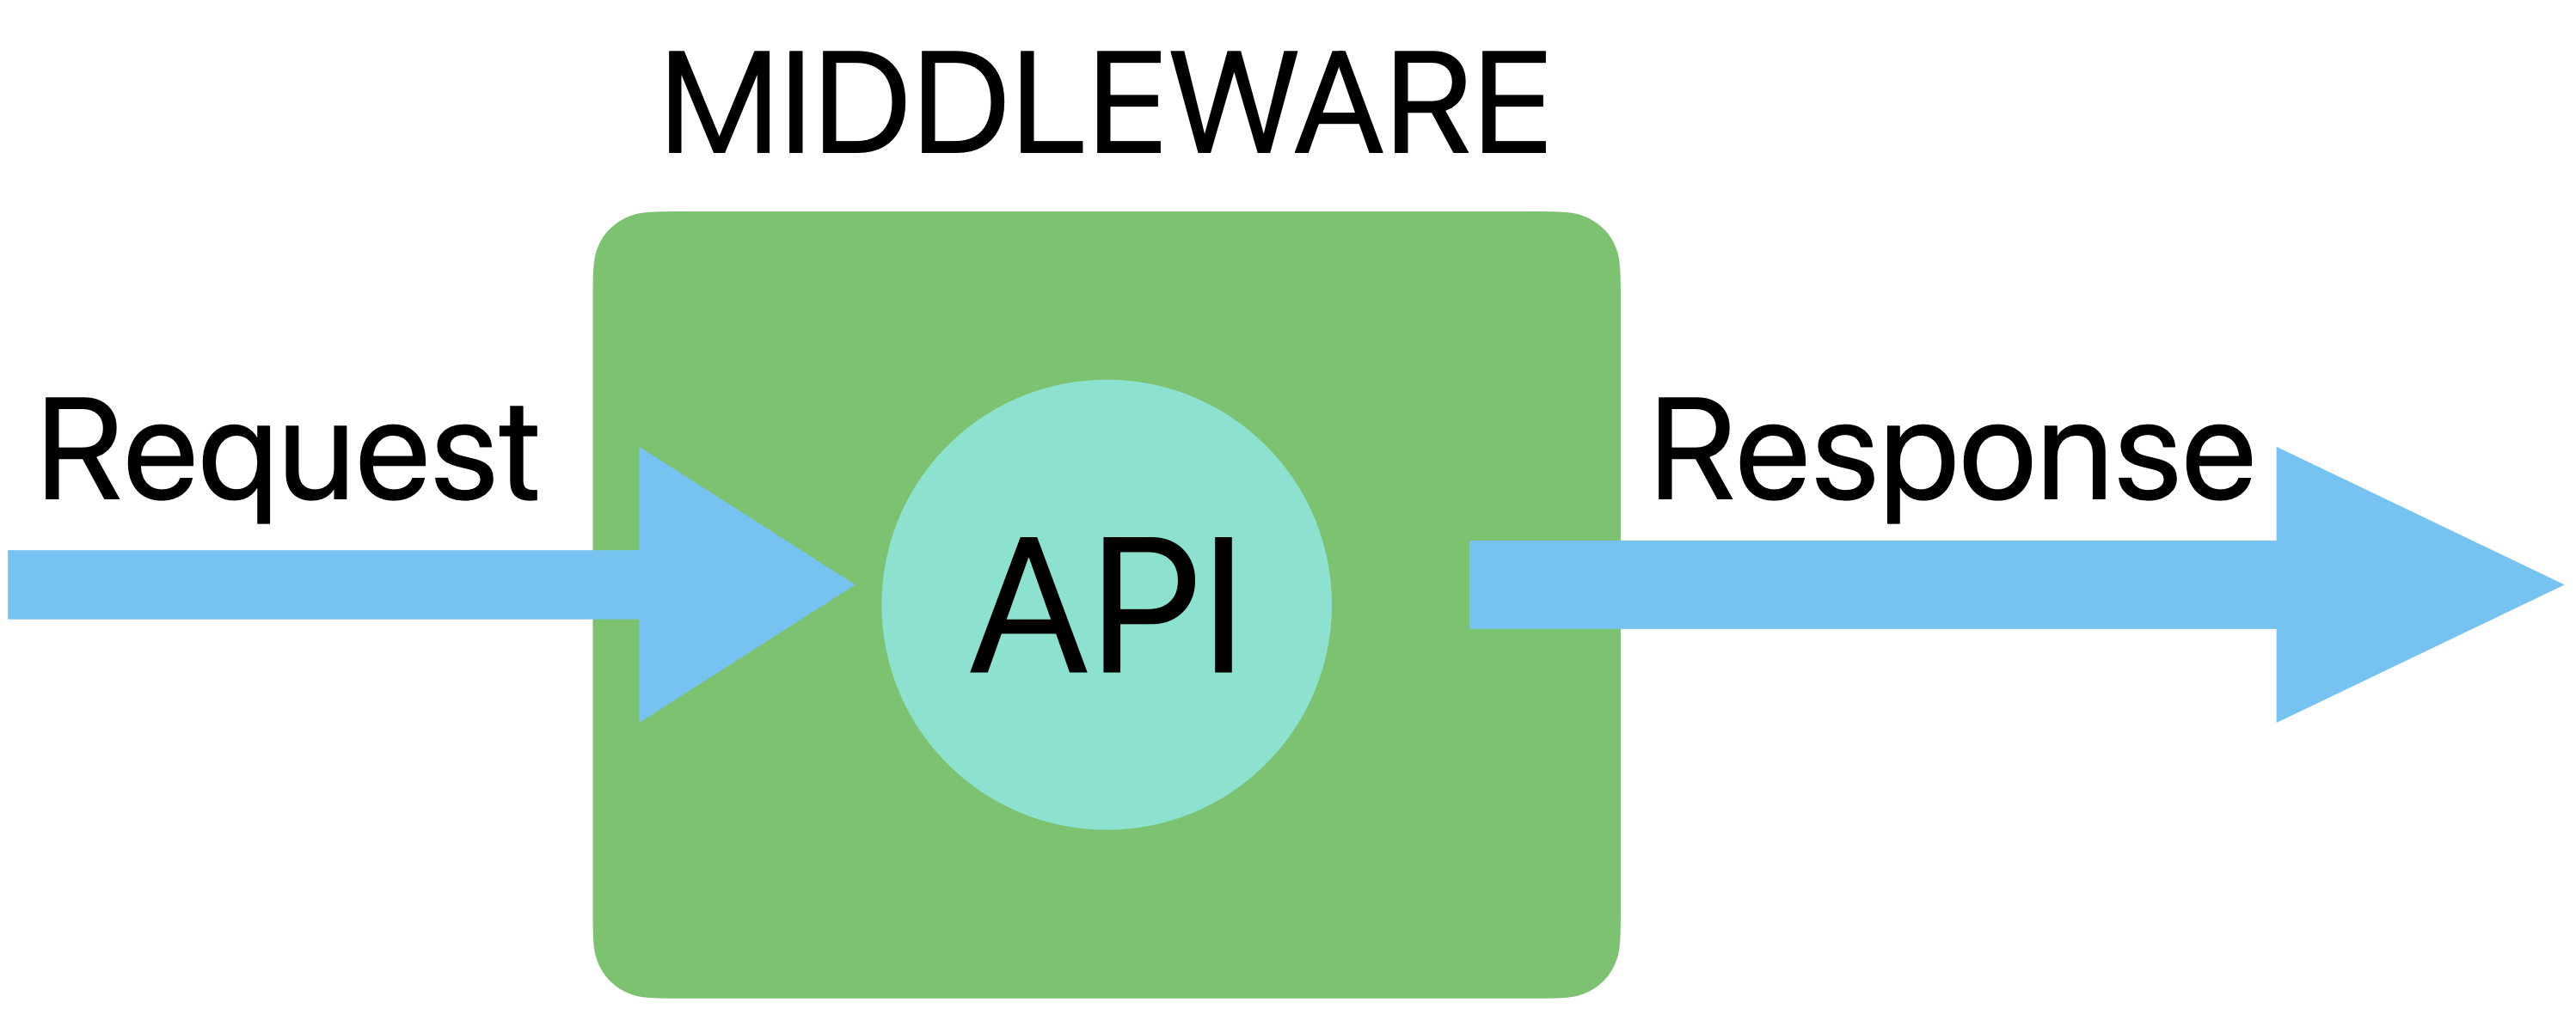
\includegraphics[width=250px]{img/ExpressJS_Middleware_1.png}
	\caption{ExpressJS Middleware}
\end{figure}
Eine Middleware-Funktion enthält in der Regel das Anfrageobjekt, das Antwortobjekt und die Middleware-Funktion selbst. Middleware kann auch die Antwort an den Server senden, bevor die Anfrage abgeschlossen ist. Die nächste Middleware-Funktion wird normalerweise als Variable mit dem Namen "next" dargestellt. Im Grunde ist Middleware eine Funktion, die nur über Routen angewendet werden kann. Middleware kann auch verwendet werden, um auf Anfragen und Antworten zuzugreifen und diese zu ändern.
\\
Middleware kann mehrere Aufgaben erfüllen. Es kann beliebigen Code ausführen, Änderungen an den Anfrage-Antwort-Objekten vornehmen, den Anfrage-Antwort-Zyklus beenden oder die nächste Middleware-Funktion im Stapel aufrufen. Mit diesen Funktionen können wir Middleware modifizieren, um viele Aufgaben auszuführen, wie beispielsweise eine Website für bestimmte Länder zu sperren oder die Authentifizierung eines Benutzers zu überprüfen.
\\
Um Middleware in einer Express-Anwendung zu erstellen, können wir eine separate Middleware-Datei erstellen und diese ausführen. Dazu müssen wir zunächst alle Pakete installieren, die für die Ausführung von Express-Middleware benötigt werden. Anschließend können wir die Middleware-Datei erstellen und ausführen, um die Funktionen der Middleware in unserer Anwendung zu nutzen.
\\
Im Beispiel wird gezeigt, wie eine Middleware-Funktion in Express erstellt werden kann. Zunächst wird eine einfache Express-\acs{API} erstellt und dann eine Middleware-Datei erstellt. In dieser Datei wird die Middleware-Funktion definiert, die aufgerufen wird, wenn eine Anfrage an die \acs{API} gestellt wird. Die Middleware-Funktion ruft dann die nächste Middleware-Funktion auf und gibt die Antwort an den Client zurück.
\\
Insgesamt bietet Middleware eine einfache Möglichkeit, um verschiedene Funktionen in eine Anwendung zu integrieren und diese zu verwalten. Durch die Verwendung von Middleware können Entwickler schnell und einfach Funktionen hinzufügen oder entfernen, um die Funktionalität ihrer Anwendungen zu verbessern.

\subsection{Der Grund für die Verwendung von Session}\label{appendix:a6}\par
In der Webentwicklung ist die Verwendung von Sessions ein wichtiger Aspekt bei der Entwicklung von Überwachungssystemen. Eine Session ermöglicht es, den Benutzer während seiner Interaktion mit dem System zu identifizieren und seine Aktionen zu verfolgen. Dies ist besonders wichtig bei der Überwachung eines komplexen Systems, bei dem viele Komponenten beteiligt sind.
\\
Durch die Verwendung von Sessions kann der Benutzer authentifiziert werden, um sicherzustellen, dass nur autorisierte Benutzer auf das System zugreifen können. Außerdem kann die Session genutzt werden, um die Berechtigungen des Benutzers zu überprüfen und sicherzustellen, dass er nur auf die Bereiche des Systems zugreifen kann, auf die er zugreifen sollte.
\\
Eine Session ermöglicht auch die Verfolgung der Aktivitäten des Benutzers im System, was hilfreich sein kann, um ungewöhnliches Verhalten oder mögliche Sicherheitsbedrohungen zu erkennen. Durch die Aufzeichnung von Benutzeraktivitäten in der Session können Probleme schneller erkannt und behoben werden.

\subsection{Der Grund für die Verwendung von Helmet.js}\label{appendix:a7}\par
Helmet.js ist ein Middleware-Modul für Express, das verschiedene \acs{HTTP}-Header für verbesserte Sicherheit konfiguriert. Es ist wichtig für die Webentwicklung, insbesondere für Systeme zur Überwachung, da es dazu beiträgt, Angriffe auf die Anwendung zu verhindern und die Sicherheit zu erhöhen. Einige der Funktionen, die Helmet.js bietet, sind:
\begin{itemize}
	\item \textbf{XSS-Schutz:} Cross-Site-Scripting-Angriffe können durch Einfügen von Skripten in die Benutzereingabe durchgeführt werden. Helmet.js konfiguriert den X-XSS-Protection-Header, um solche Angriffe zu blockieren.
	\item \textbf{HTTP-Header-Steuerung:} \acs{HTTP}-Header können so konfiguriert werden, dass sie Angriffe verhindern oder abmildern. Beispielsweise kann der X-Content-Type-Options-Header so eingestellt werden, dass der Browser dazu gezwungen wird, nur MIME-Typen zu akzeptieren, die der Server ausdrücklich angibt.
	\item \textbf{Clickjacking-Schutz:} Clickjacking-Angriffe können dazu führen, dass Benutzer auf unerwünschte Links klicken, ohne es zu merken. Helmet.js konfiguriert den X-Frame-Options-Header, um solche Angriffe zu verhindern.
	\item \textbf{Weitere Funktionen:} Weitere Funktionen von Helmet.js sind das Verhindern von MIME-Sniffing, das Verbergen von X-Powered-By-Headern und das Hinzufügen von Strict-Transport-Security-Headern.
\end{itemize}

\clearpage

\subsection{Fehlercodes und Statuscode-Meldungen}\label{appendix:a8}\par
In der Webentwicklung ist es von großer Bedeutung,
standardisierte Fehlercodes und Statuscode-Meldungen zu verwenden, da sie dazu beitragen, Fehler schnell zu erkennen und zu beheben. Eine Tabelle, die diese Codes und Meldungen enthält (siehe Abbildung 2), ist eine nützliche Referenz, um Fehler zu identifizieren und zu beheben. Die Tabelle sollte alle relevanten Codes enthalten, die von der Anwendung verwendet werden, sowie eine kurze und klare Beschreibung der zugehörigen Meldungen. Es ist auch wichtig, dass die Codes und Meldungen präzise formuliert sind, um eine einfache Verständlichkeit zu gewährleisten.
\begin{figure}[htbp]
	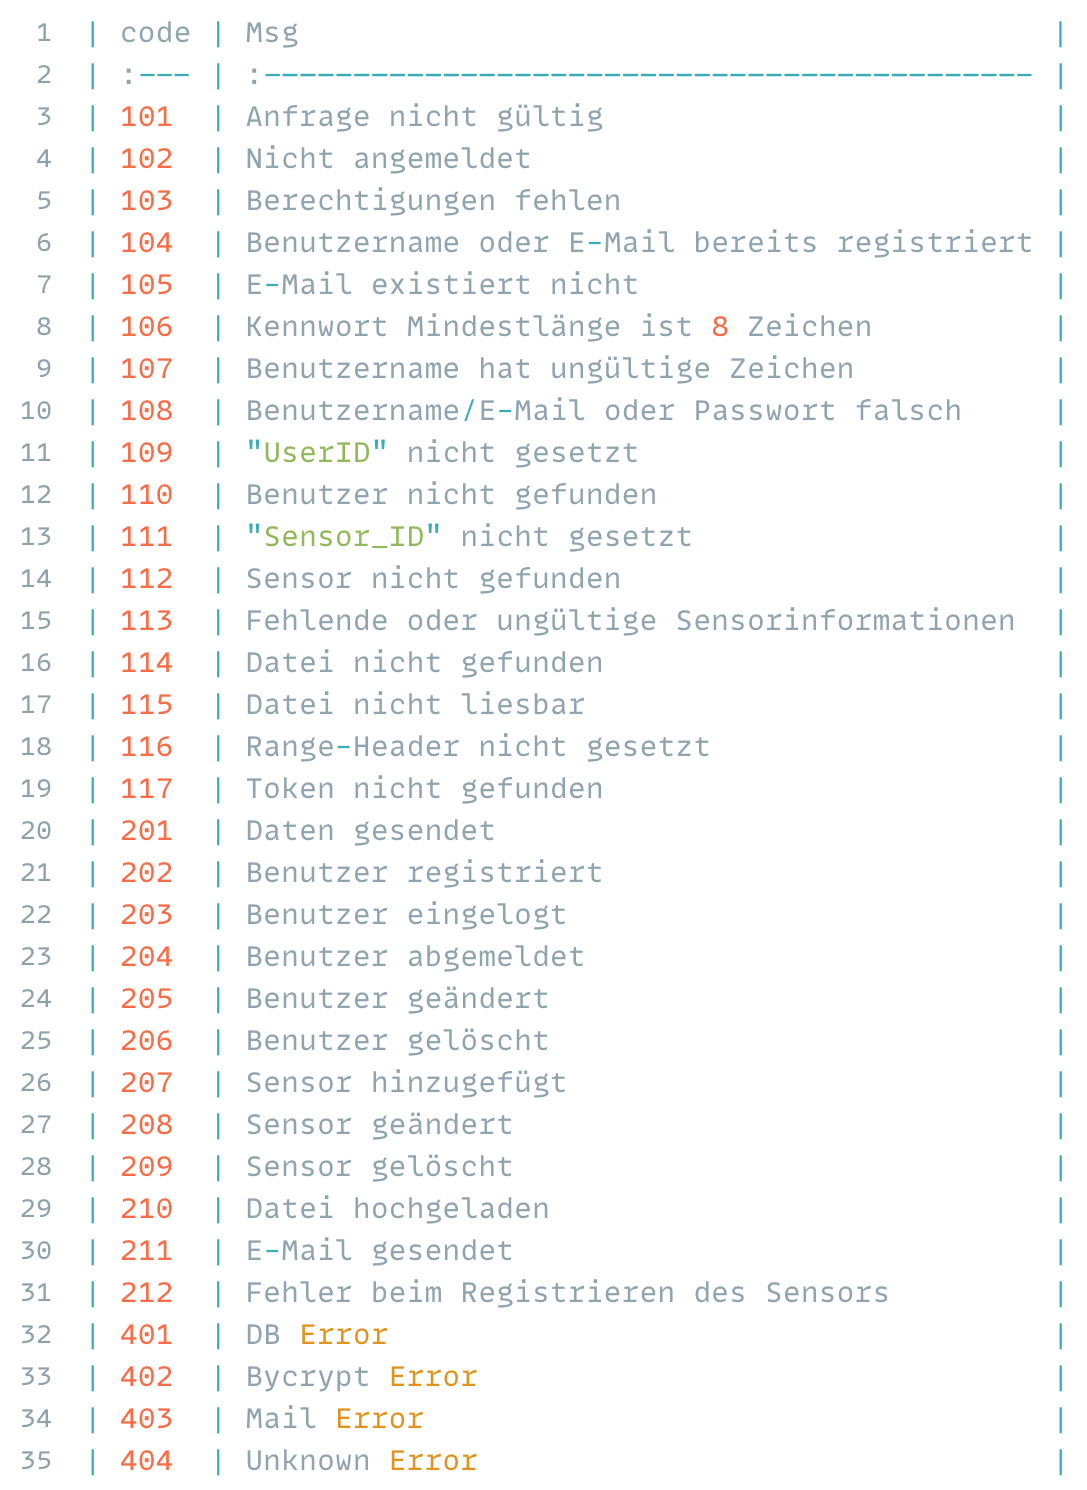
\includegraphics[width=300px]{img/Statuscode-Meldungen.png}
	\caption{Fehlercodes und Statuscode-Meldungen}
\end{figure}

\clearpage

\subsection{Use-case Diagramm}\label{appendix:a9}\par
\begin{figure}[htbp]
	\centering
	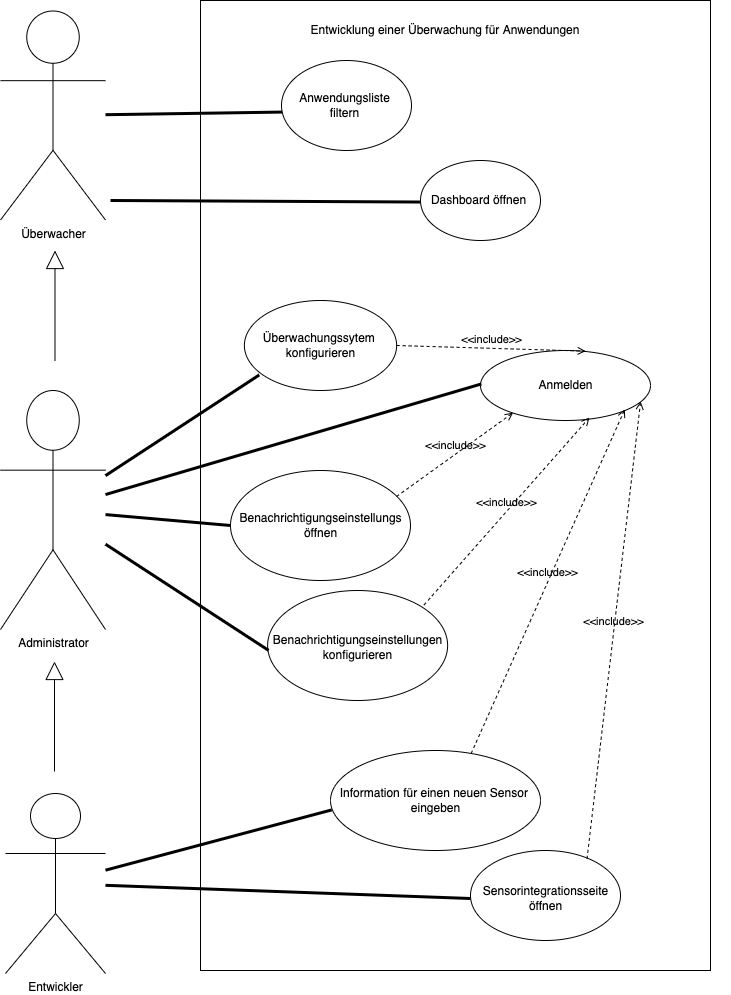
\includegraphics[width=300px]{img/anwendungsfalldiagramm.png}
	\caption{Use-case Diagramm}
\end{figure}
\clearpage



\subsection{Komponenten Diagramm}\label{appendix:a10}\par
\begin{figure}[htbp]
	\centering
	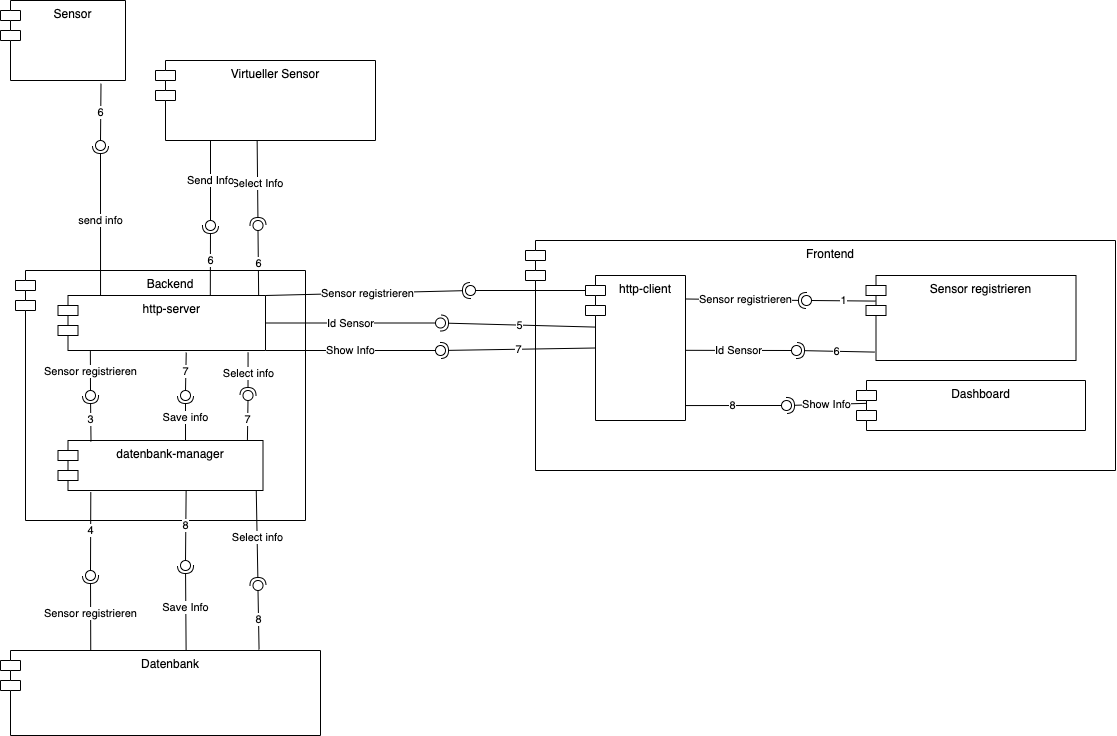
\includegraphics[width=1\textwidth]{img/komponent_diagram.png}
	\caption{Komponenten Diagramm}
\end{figure}
\clearpage

\section{Relationales Datenbankmodell}\label{appendix:b}\par

Für dieses Projekt wurde ein Entity-Relationship-Diagramm (ER-Diagramm) erstellt, um die Struktur der Datenbank und die Beziehungen zwischen den verschiedenen Entitäten zu modellieren. Das ER-Diagramm bildet die Grundlage für das Datenbankschema und hilft bei der Organisation der Daten, die im Rahmen des Überwachungssystems erfasst und verarbeitet werden.
\begin{figure}[h]
	\centering
	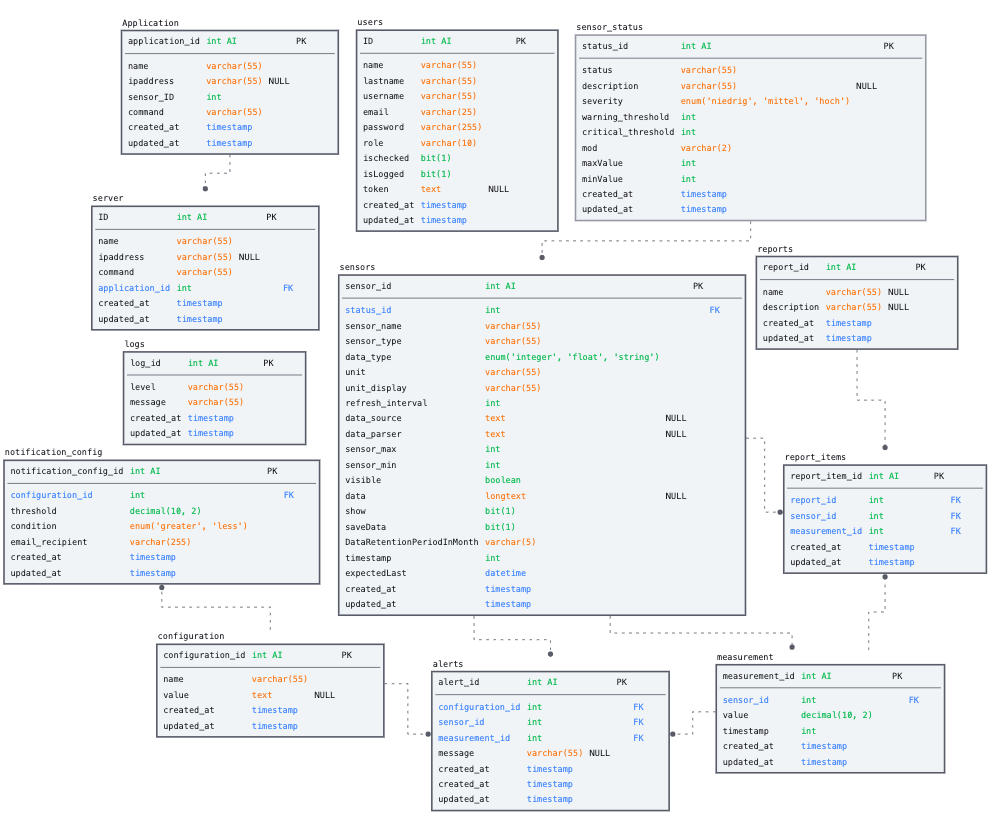
\includegraphics[width=1\textwidth]{img/ERP-diagramm.png}
	\caption{Relationales Datenbankmodell}
	\label{Relationales Datenbankmodell}
\end{figure}
\clearpage

\subsection{Screenshot des Sprint-Boards in GitHub}\label{appendix:b1}\par


In diesem Projekt wurde ein Sprint-Board in GitHub für die Planung und Verwaltung der Softwareentwicklung eingesetzt. Das Kanban Board ermöglichte eine effektive Organisation der verschiedenen Aufgaben und Phasen des Projekts, indem es den Fortschritt in Echtzeit darstellte. Als Einzelperson war das Kanban Board ein wertvolles Instrument zur Selbstorganisation und zum Nachverfolgen der Aufgaben, um sicherzustellen, dass alle notwendigen Schritte abgeschlossen und Ziele erreicht wurden.

\begin{figure}[htbp]
	\centering
	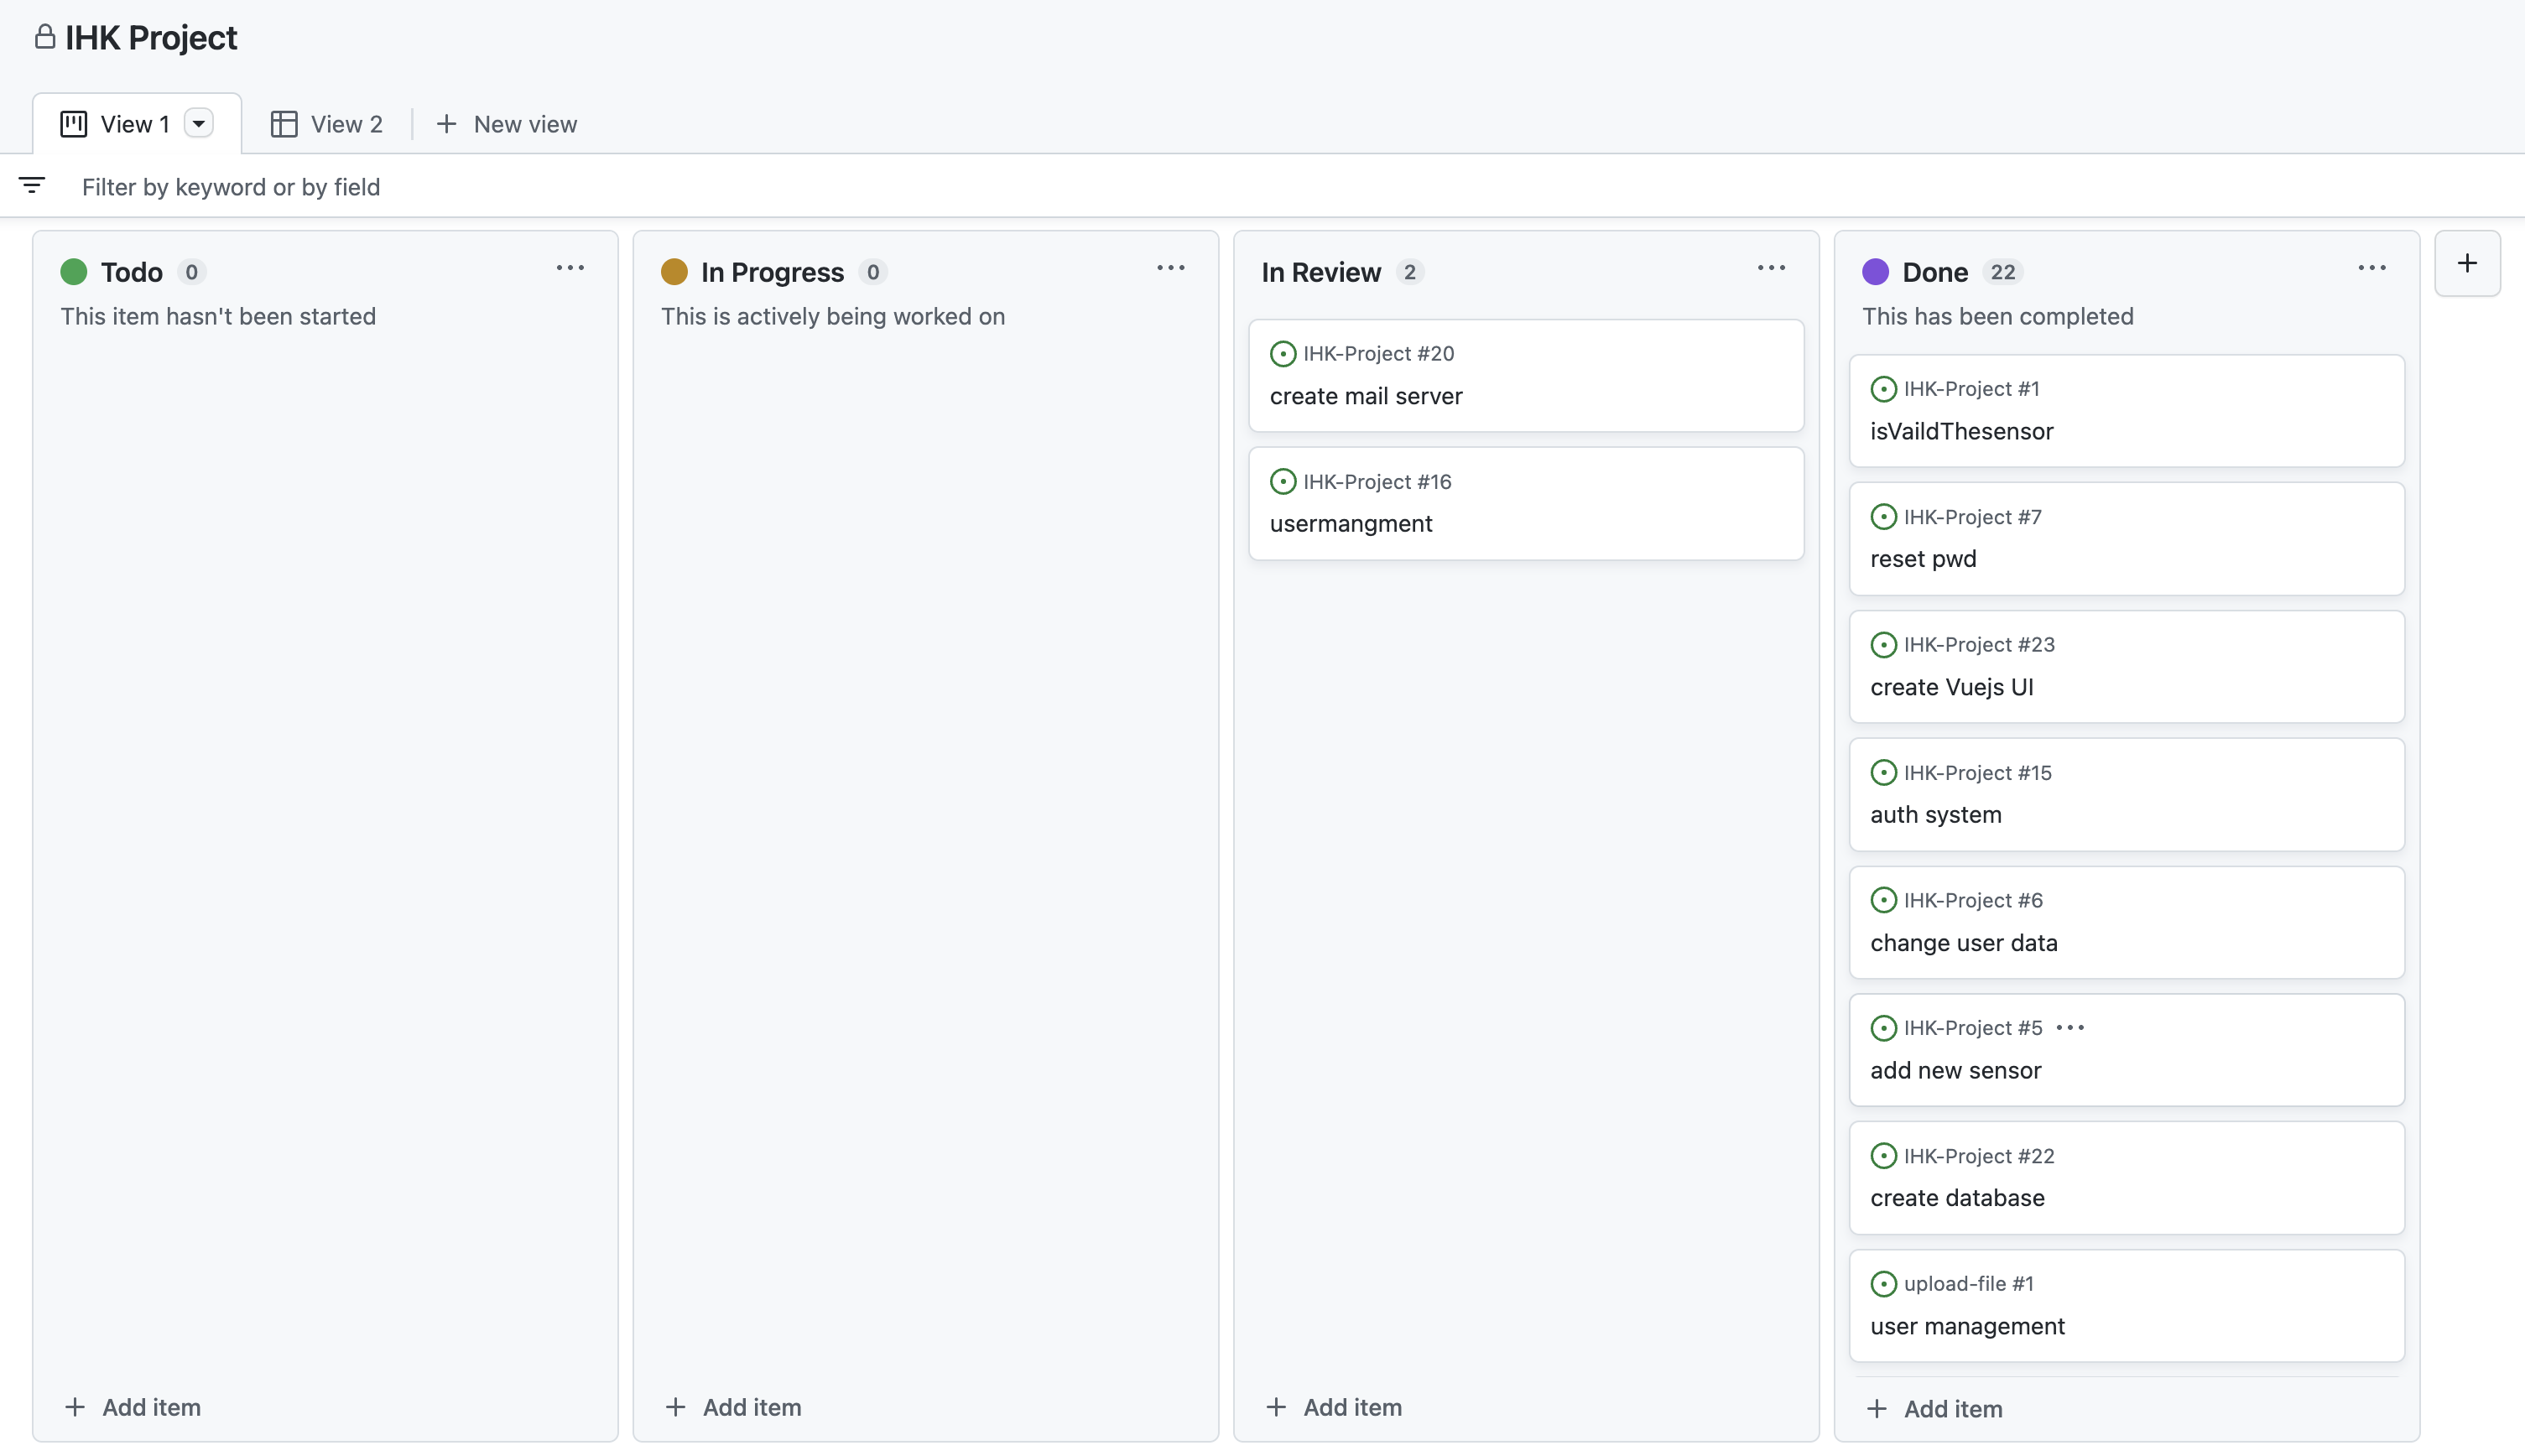
\includegraphics[width=1\textwidth]{img/github_canban.png}
	\caption{Screenshot des Sprint-Boards in GitHub}
	\label{Screenshot des Sprint-Boards in GitHub}
\end{figure}
\clearpage

\subsection{Verwendung von Gantt-Diagramm in GitHub für die Projektplanung}\label{appendix:b2}\par

Seitdem GitHub die Unterstützung für Gantt-Diagramme in seinem Feature-Set integriert hat, ist die Planung und Verfolgung von Projekten einfacher geworden. Durch die Verwendung von Gantt-Diagrammen in GitHub können die verschiedenen Phasen des Projekts, Meilensteine und Aufgaben übersichtlich dargestellt und der Fortschritt sowie die Abhängigkeiten zwischen den einzelnen Aufgaben verfolgt werden. Dies trägt zur effektiven Planung, Zeitmanagement und zur rechtzeitigen Erreichung der Projektziele bei.
\begin{figure}[htbp]
	\centering
	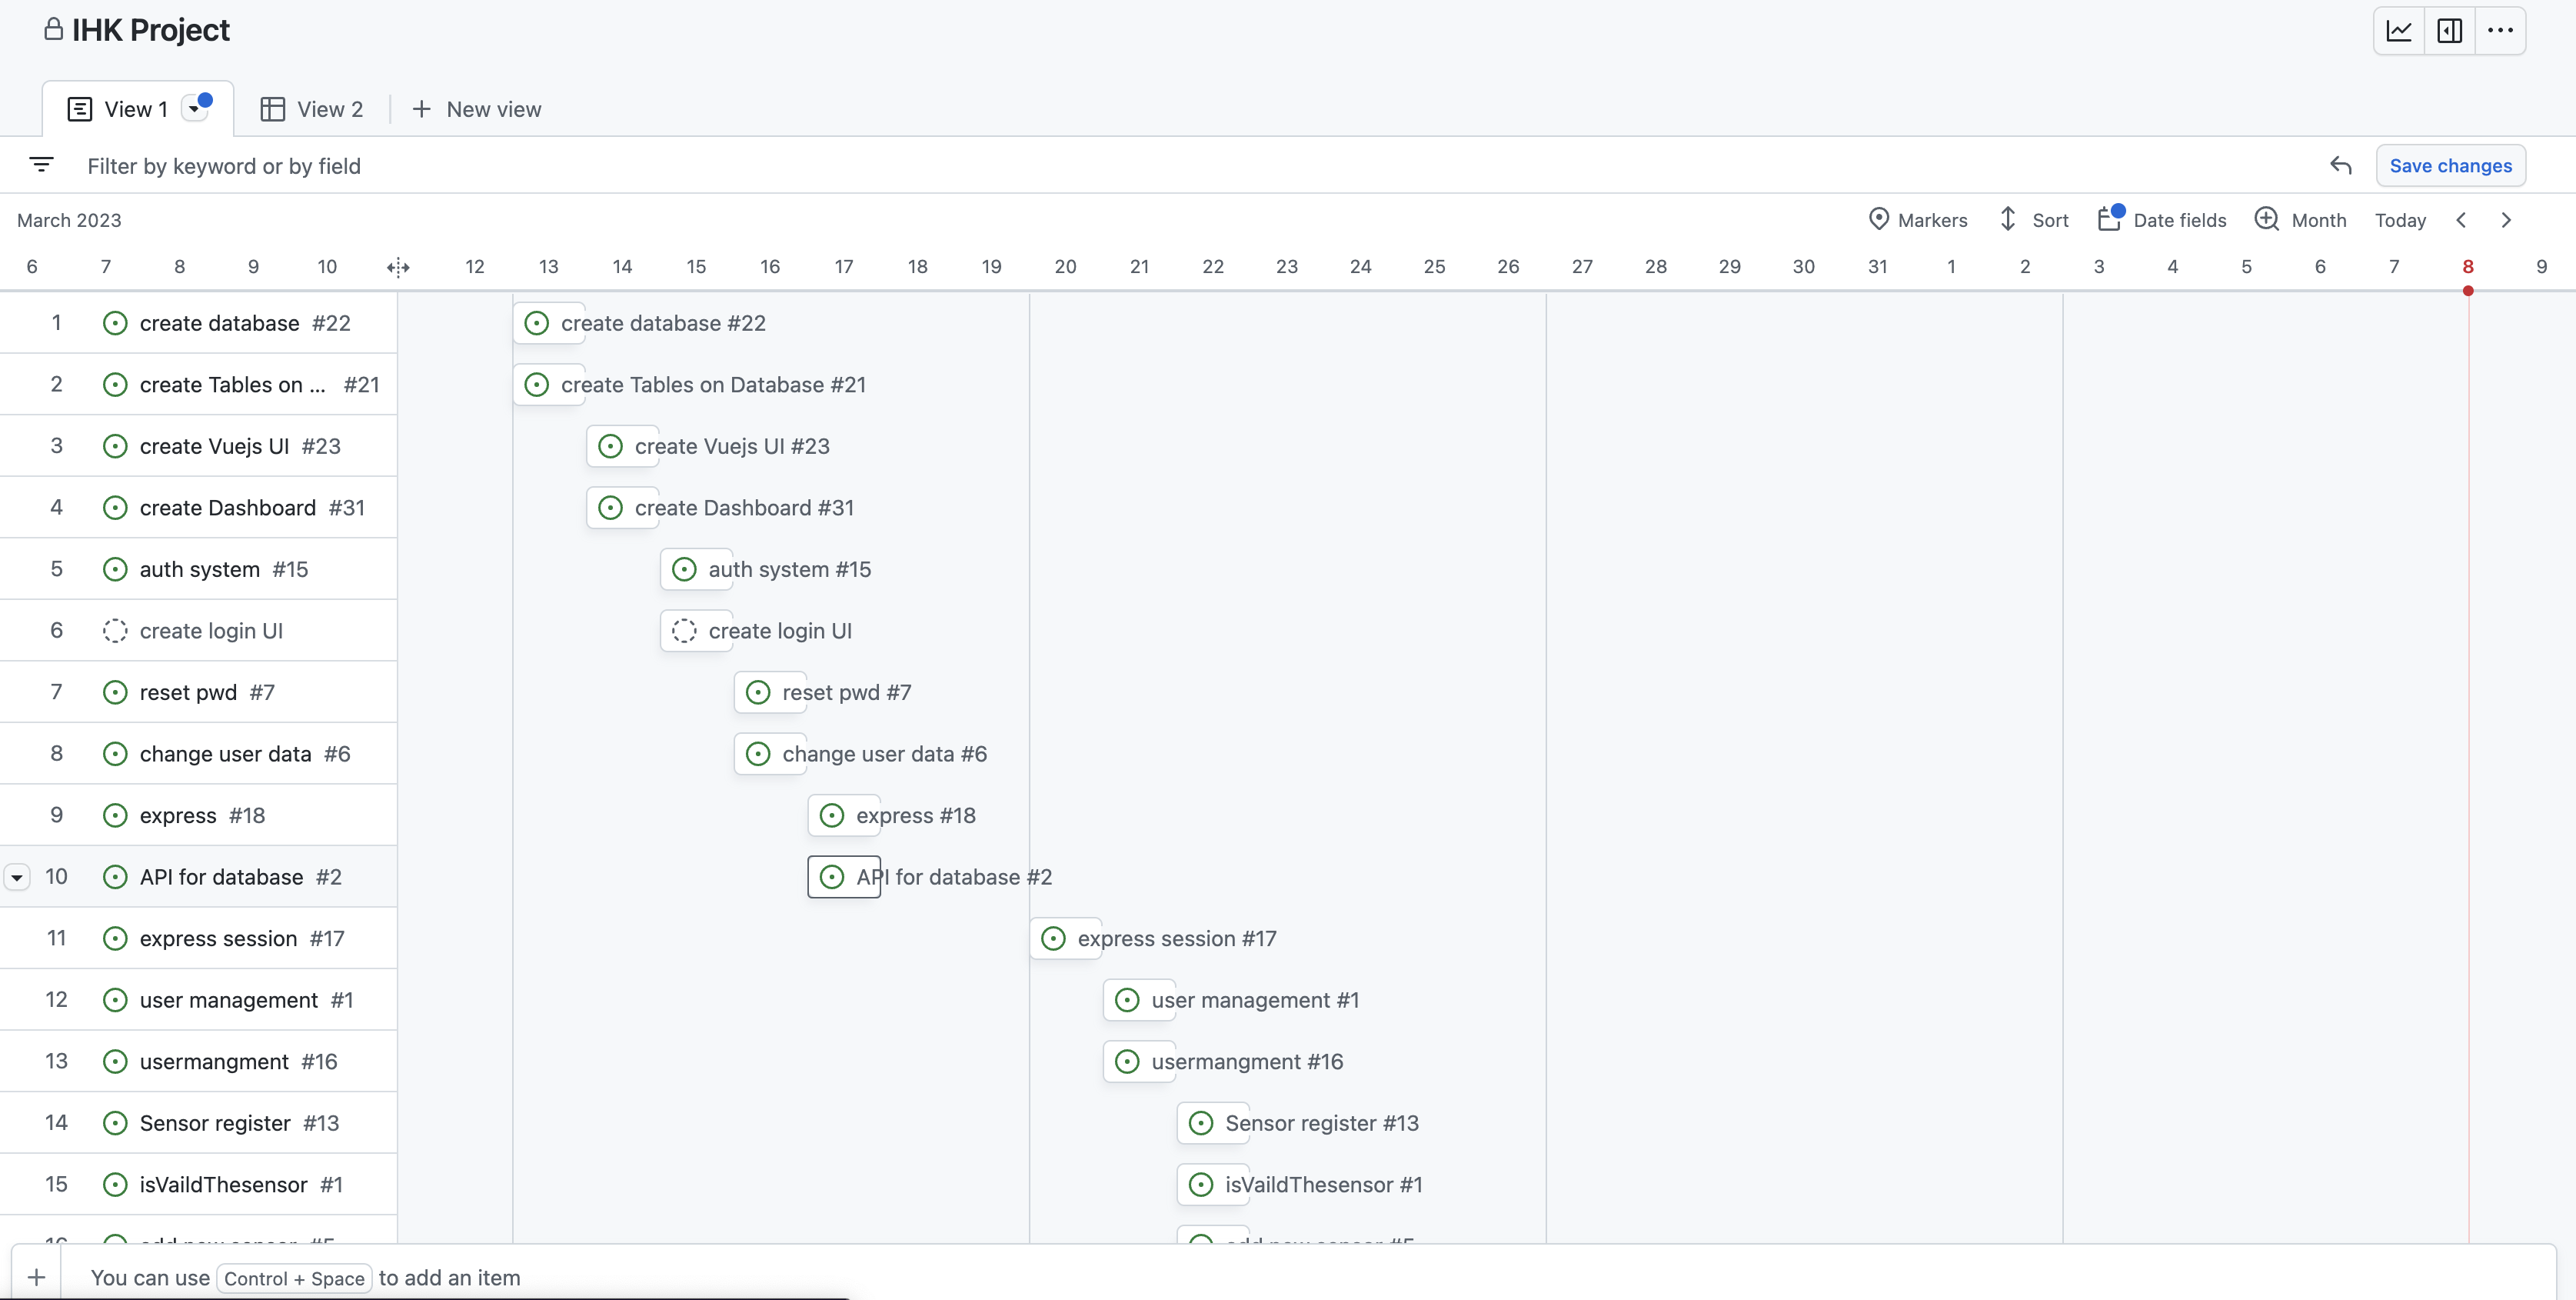
\includegraphics[width=1\textwidth]{img/github_diaramm.png}
	\caption{Verwendung von Gantt-Diagramm in GitHub für die Projektplanung}
	\label{Verwendung von Gantt-Diagramm in GitHub für die Projektplanung}
\end{figure}
\clearpage

\subsection{Screenshot des File-Trees Backend}\label{appendix:b5}\par
Das Projekt wurde mit einer sorgfältig durchdachten Ordnerstruktur als Back-End entwickelt, um eine hohe Organisationsstruktur und Fehlerfreiheit zu gewährleisten.
Durch die präzise Aufteilung der Dateien und Verzeichnisse ist es einfach, Probleme zu finden und zu beheben.
Auf diese Weise können wir eine reibungslose Funktionsweise unseres Produkts sicherstellen und die Benutzererfahrung optimieren.
\begin{figure}[htbp]
	\centering
	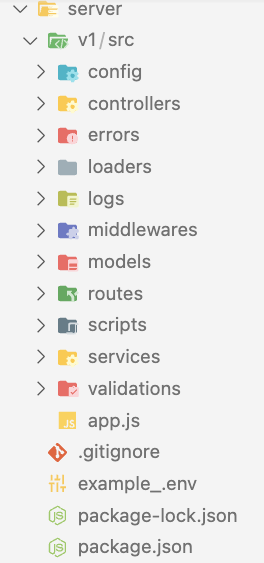
\includegraphics[width=100px]{img/vsd.png}
	\caption{Screenshot des File-Trees Backend}
\end{figure}
\clearpage


\subsection{Anmeldung eines neuen Sensors}\label{appendix:b3}\par
Im folgenden Abschnitt wird ein \acs{JSON} beschrieben, das einen Sensor mit dem Datentyp “integer” repräsentiert.


Mit diesem \acs{JSON} kann der Sensor seine Daten und Einstellungen an das Backend senden, um beispielsweise Daten an das Frontend zu senden oder die Daten in der Datenbank zu speichern. Das Backend verwendet diese Informationen, um den Sensor zu verwalten und seine Konfiguration zu aktualisieren.
	\begin{lstlisting}[caption={Anmeldung eines neuen Sensors (Backend)  JSON-Modell}, style=js]
		{
			sensor_name: 'Anrufe pro Stunde',
			sensor_type: 'process',
			data_type: 'integer',
			unit: 'anrufe',
			unit_display: 'Anrufe/h',
			refresh_interval: 60,
			data_source: 'htts://192.168.12.31:4000',
			data_parser: '',
			sensor_max: 1000,
			sensor_min: 0,
			show: true,
			saveData: true,
			DataRetentionPeriodInMonths: 6,
			visible: true,
			Data: ''
		}
	\end{lstlisting}
\clearpage



	\begin{lstlisting}[caption={Anmeldung eines neuen Sensors (Backend)}, style=js]
		// Function to validate if all required fields are present in the sensor data object
		const validateSensorData = (sensorData) => {
			// List of all required fields
			const requiredFields = [
				"sensor_name",
				"sensor_type",
				"data_type",
				"unit",
				"unit_display",
				"refresh_interval",
				"data_source",
				"data_parser",
				"sensor_max",
				"sensor_min",
				"visible",
				"Data",
				"show",
				"saveData",
				"DataRetentionPeriodInMonths",
			];

			// Check if each required field exists in the sensor data object
			// If any required field is missing, return false
			requiredFields.forEach((field) => {
				if (!sensorData.hasOwnProperty(field)) {
					return false;
				}
			});

			// If all required fields are present, return true
			return true;
		};

		// Route to register a new sensor
		app.post('/registerSensor', async (req, res) => {
			const sensorData = req.body;

			// Validate if all required fields are present in the sensor data object
			if (!validateSensorData(sensorData)) {
				// If any required field is missing, return an error response
				res.status(400).json({
					code: 113,
					message: 'Fehlende oder ungueltige Sensorinformationen',
				});
				return;
			}

			// Add the sensor to the database
			try {
				// Establish a database connection
				const connection = await db.getConnection();

				// SQL query to insert the sensor data into the database
				const sql = `
				INSERT INTO sensors (sensor_name, sensor_type, data_type, unit, unit_display, refresh_interval, data_source, sensor_max, sensor_min, visible, data, show, saveData, DataRetentionPeriodInMonths)
				VALUES (?, ?, ?, ?, ?, ?, ?, ?, ?, ?, ?, ?, ?, ?, ?);
			 `;

				// Parameters for the SQL query
				const params = [
					sensorData.sensor_name,
					sensorData.sensor_type,
					sensorData.data_type,
					sensorData.unit,
					sensorData.unit_display,
					sensorData.refresh_interval,
					sensorData.data_source,
					sensorData.data_parser,
					sensorData.sensor_max,
					sensorData.sensor_min,
					sensorData.visible,
					sensorData.Data || '',
					sensorData.show,
					sensorData.saveData,
					sensorData.DataRetentionPeriodInMonths,
				];

				// Execute the SQL query
				const result = await connection.query(sql, params);

				// Get the sensor ID of the newly inserted sensor
				const sensorId = result.insertId;

				// Close the database connection
				await connection.end();

				// Send a success response with the sensor ID
				res.status(201).json({
					message: 'Sensor erfolgreich registriert',
					code: 207,
					sensor_id: sensorId,
				});
			} catch (error) {
				// If there is an error while adding the sensor, return an error response
				console.error('Error adding sensor:', error);
				res.status(500).json({
					message: 'Fehler beim Registrieren des Sensors',
					code: 212,
				});
			}
		});
	\end{lstlisting}
\clearpage


	\begin{lstlisting}[caption={Anmeldung eines neuen Sensors (Backend) Unit-Tests}, style=js]
		describe('Sensor API Tests', () => {
			it('should register a new sensor', async () => {
				const sensorData = {
					sensor_name: 'Anrufe pro Stunde',
					sensor_type: 'process',
					data_type: 'integer',
					unit: 'anrufe',
					unit_display: 'Anrufe/h',
					refresh_interval: 60,
					data_source: 'htts://192.168.12.31:4000',
					data_parser: '',
					sensor_max: 1000,
					sensor_min: 0,
					show: true,
					DataRetentionPeriodInMonths: 6,
					visible: true,
					Data: ''
				};
				const res = await request(app).post('/registerSensor').send(sensorData);
				expect(res.statusCode).toEqual(201);
				expect(res.body.message).toEqual('Sensor erfolgreich registriert');
				expect(res.body.sensor_id).toBeDefined();
			});

			it('should return an error message if sensor data is incomplete', async () => {
				const sensorData = {
					sensor_name: 'Anrufe pro Stunde',
					sensor_type: 'process',
					data_type: 'integer',
					unit: 'anrufe',
					unit_display: 'Anrufe/h',
					refresh_interval: 60,
					data_source: 'htts://192.168.12.31:4000',
					data_parser: '',
					sensor_max: 1000,
					sensor_min: 0,
					show: true
				};
				const res = await request(app).post('/registerSensor').send(sensorData);
				expect(res.statusCode).toEqual(400);
				expect(res.body.message).toEqual('Fehlende oder ungueltige Sensorinformationen');
			});
		});
	\end{lstlisting}
\clearpage


\begin{figure}[htbp]
	\centering
	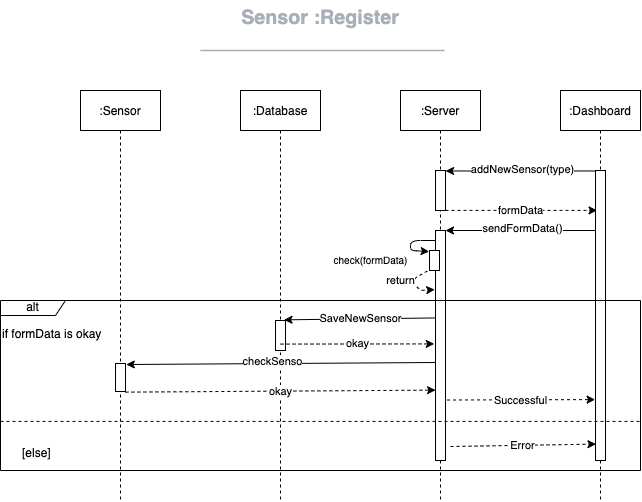
\includegraphics[width=1\textwidth]{img/register_sequence_Diagramm.png}
	\caption{Anmeldung eines neuen Sensors Sequenzdiagramm}
\end{figure}
\clearpage

\subsection{Sequenzdiagramm: Sensor schickt Daten}\label{appendix:b4}\par

In diesem Sequenzdiagramm wird dargestellt, wie der Sensor Daten an den Server sendet und wie der Server die Daten in der Datenbank speichert. Außerdem wird gezeigt, wie das Dashboard die Daten aktualisiert:
\begin{itemize}
	\item Der Sensor erfasst Daten und sendet sie an den Server.
	\item Der Server empfängt die Daten und verarbeitet sie.
	\item Der Server speichert die verarbeiteten Daten in der Datenbank.
	\item Das Dashboard fordert regelmäßig aktualisierte Daten von der Datenbank an.
	\item Der server sendet die angeforderten Daten an das Dashboard.
	\item Das Dashboard aktualisiert die angezeigten Daten entsprechend den neuen Daten.
\end{itemize}

Durch diese Darstellung wird der Datenfluss von der Erfassung durch den Sensor bis zur Anzeige auf dem Dashboard verdeutlicht.

\begin{figure}[h]
	\centering
	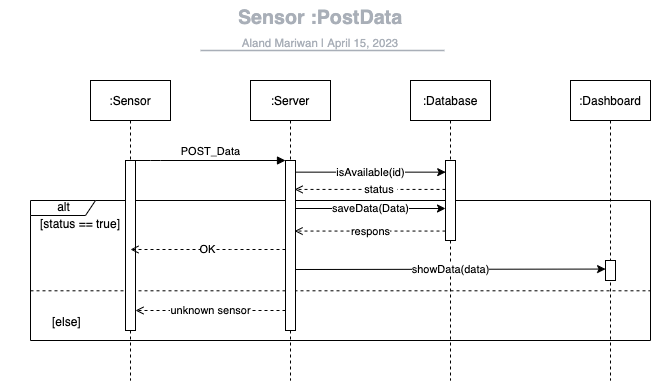
\includegraphics[width=1\textwidth]{img/postData_sequence_Diagramm.png}
	\caption{Sensor schickt Daten (Sequenzdiagramm)}
\end{figure}
\clearpage




\begin{lstlisting}[caption={Sensor schickt Daten (Backend)}, style=js]
	router.get('sensor/:id/data', async (req, res) => {
		try {
			const sensorId = req.params.id;
			const sensor = await db.getSensorById(sensorId);
			if (!sensor) {
				res.status(404).json({
					message: 'Sensor nicht gefunden',
					code: 112,
				});
				return;
			}
			const data = await db.getLastestSensorData(sensorId);
			if (!data) {
				res.status(204).json({
					message: 'Keine Daten vorhanden',
					code: 113,
				});
				return;
			}
			res.status(200).json({
				data: data,
				message: 'Daten gesendet',
				code: 201,
			});
		} catch (err) {
			console.error(err);
			res.status(500).json({ message: 'DB Error', code: 401 });
		}
	});
\end{lstlisting}

	\begin{lstlisting}[caption={Sensor schickt Daten (Backend) Unit-Tests }, style=js]

		describe('GET /sensor/:id/data', () => {
			beforeEach(() => {
			  jest.spyOn(db, 'getSensorById').mockImplementation(async (id) => {
				 if (id === '123') {
					return { id: '123', name: 'Test Sensor' };
				 }
				 return null;
			  });

			  jest.spyOn(db, 'getLastestSensorData').mockImplementation(async (id) => {
				 if (id === '123') {
					return { id: '456', sensorId: '123', value: 10 };
				 }
				 return null;
			  });
			});

			afterEach(() => {
			  jest.restoreAllMocks();
			});

			it('should return 404 if sensor not found', async () => {
			  const res = await request(app).get('/sensor/456/data');

			  expect(res.status).toBe(404);
			  expect(res.body.message).toBe('Sensor nicht gefunden');
			  expect(res.body.code).toBe(112);
			});

			it('should return 204 if no data available', async () => {
			  const res = await request(app).get('/sensor/123/data');

			  expect(res.status).toBe(204);
			  expect(res.body.message).toBe('Keine Daten vorhanden');
			  expect(res.body.code).toBe(113);
			});

			it('should return latest data for the sensor', async () => {
			  const res = await request(app).get('/sensor/123/data');

			  expect(res.status).toBe(200);
			  expect(res.body.message).toBe('Daten gesendet');
			  expect(res.body.code).toBe(201);
			  expect(res.body.data.id).toBe('456');
			  expect(res.body.data.sensorId).toBe('123');
			  expect(res.body.data.value).toBe(10);
			});

			it('should handle database errors', async () => {
			  jest.spyOn(db, 'getSensorById').mockImplementation(async () => {
				 throw new Error('Database error');
			  });

			  const res = await request(app).get('/sensor/123/data');

			  expect(res.status).toBe(500);
			  expect(res.body.message).toBe('DB Error');
			  expect(res.body.code).toBe(401);
			});
		 });
	\end{lstlisting}
\clearpage




	\begin{lstlisting}[caption={Neue Benutzer hinzufügen (Backend)}, style=js]
		router.post('/register', function (req, res) {
			let name = decrypt(req.body.name);
			let lastname = decrypt(req.body.lastname);
			let username = decrypt(req.body.username);
			let email = decrypt(req.body.email);
			let password = decrypt(req.body.password);

			if (
				name === false ||
				lastname === false ||
				username === false ||
				email === false ||
				password === false
			) {
				res.status(400).send({
					msg: 'Anfrage nicht gueltig',
					code: 101,
				});
				return;
			}
			username = username.toLowerCase();
			email = email.toLowerCase();

			if (!isEmail(email)) {
				res.status(400).send({
					msg: 'E-Mail existiert nicht',
					code: 105,
				});
				return;
			}

			if (!checkUsername(username)) {
				res.status(400).send({
					msg: 'Benutzername hat ungueltige Zeichen',
					code: 107,
				});
				return;
			}

			if (password.length < 8) {
				res.status(400).send({
					msg: 'Kennwort Mindestlaenge ist 8 Zeichen',
					code: 106,
				});
				return;
			}

			db.query(
				'SELECT * FROM users WHERE username = ? OR email = ?',
				[username, email],
				function (err, result) {
					if (err) {
						console.error(err);
						res.status(500).send({
							msg: 'DB Error',
							code: 401,
							err: err,
						});
						return;
					}

					if (result.length != 0) {
						res.status(500).send({
							msg: 'Benutzername oder E-Mail bereits registriert',
							code: 104,
						});
						return;
					}

					bcrypt.hash(password, saltRounds, function (err2, hash) {
						if (err2) {
							console.error(err2);
							res.status(500).send({
								msg: 'Bycrypt Error',
								code: 402,
								err: err2,
							});
							return;
						}

						db.query(
							'INSERT INTO users (name, lastname, username, email, password ) VALUE (?,?,?,?,?)',
							[name, lastname, username, email, hash],
							function (error, response) {
								if (error) {
									console.error(error);
									res.status(500).send({
										msg: 'DB Error',
										code: 401,
										err: error,
									});
									return;
								}

								res.status(200).send({
									msg: 'Benutzer registriert',
									code: 202,
								});
							},
						);
					});
				},
			);
		});
	\end{lstlisting}
\clearpage

	\begin{lstlisting}[caption={Neue Benutzer hinzufügen (Backend) Unit-Tests}, style=js]
		describe('POST /auth/register', () => {
			test('should return 400 if request is invalid', async () => {
				var nameHash = encrypt('invalid');
				var lastnameHash = encrypt('request');
				var usernameHash = encrypt('invalid');
				var emailHash = encrypt('invalid');
				var passwordHash = bcrypt.hashSync('short', saltRounds); // hash created
				const response = await request(app)
					.post('/auth/register')
					.send({
						name: nameHash,
						lastname: lastnameHash,
						username: usernameHash,
						email: emailHash,
						password: passwordHash,
					})
					.set('Content-Type', 'application/json');

				expect(response.status).toBe(400);
				expect(response.body.msg).toBe('Anfrage nicht gueltig');
				expect(response.body.code).toBe(101);
			});

			test('should return 400 if email is invalid', async () => {
				var nameHash = encrypt('Aland');
				var lastnameHash = encrypt('Mariwan');
				var usernameHash = encrypt('amariwan');
				var emailHash = encrypt('invalid');
				var passwordHash = bcrypt.hashSync('short1234568', saltRounds); // hash created
				const response = await request(app)
					.post('/auth/register')
					.send({
						name: nameHash,
						lastname: lastnameHash,
						username: usernameHash,
						email: emailHash,
						password: passwordHash,
					})
					.set('Content-Type', 'application/json');

				expect(response.status).toBe(400);
				expect(response.body.msg).toBe('E-Mail existiert nicht');
				expect(response.body.code).toBe(105);
			});

			test('should return 400 if username has invalid characters', async () => {
				var nameHash = encrypt('Aland');
				var lastnameHash = encrypt('Mariwan');
				var usernameHash = encrypt('amariwan.99');
				var emailHash = encrypt('dev@aland-mariwan.de');
				var passwordHash = bcrypt.hashSync('short1234568', saltRounds); // hash created
				const response = await request(app)
					.post('/auth/register')
					.send({
						name: nameHash,
						lastname: lastnameHash,
						username: usernameHash,
						email: emailHash,
						password: passwordHash,
					})
					.set('Content-Type', 'application/json');

				expect(response.status).toBe(400);
				expect(response.body.msg).toBe('Benutzername hat ungueltige Zeichen');
				expect(response.body.code).toBe(107);
			});

			test('should return 400 if password is too short', async () => {
				var nameHash = encrypt('Aland');
				var lastnameHash = encrypt('Mariwan');
				var usernameHash = encrypt('amariwan.99');
				var emailHash = encrypt('dev@aland-mariwan.de');
				var passwordHash = bcrypt.hashSync('short', saltRounds); // hash created
				const response = await request(app)
					.post('/auth/register')
					.send({
						name: nameHash,
						lastname: lastnameHash,
						username: usernameHash,
						email: emailHash,
						password: passwordHash,
					})
					.set('Content-Type', 'application/json');

				expect(response.status).toBe(400);
				expect(response.body.msg).toBe('Kennwort Mindestlaenge ist 8 Zeichen');
				expect(response.body.code).toBe(106);
			});
		});
	\end{lstlisting}
\clearpage




\begin{lstlisting}[caption={Passwort zurücksetzen (Backend)}, style=js]
	// Generate a token and send it to the user's email
	const token = crypto.randomBytes(1000).toString('hex');
	const transporter = nodemailer.createTransport(config.mailAuth[0]);
	const html = fs.readFileSync('htmlMail/forgotPassword.html').toString();
	const mailOptions = {
		from: {
			name: 'GMS Passwort vergessen',
			address: config.mailAuth[0].auth.user,
		},
		to: email,
		subject: 'GMS Passwort Aenderung',
		html: html
			.replace('${__NAME__}', user.data.lastname)
			.replace('${__HOST__}', config.frontend_host)
			.replace('${__TOKEN__}', token),
	};
	transporter.sendMail(mailOptions, async (err, info) => {
		if (err) {
			console.error(err);
			res.status(400).send({
				msg: `Mail Error`,
				code: 403,
				err: err,
			});
			return;
		}
		const isSetUserTokenOnDB = await setUserTokenOnDB(token, email);
		if (isSetUserTokenOnDB.result === 0) {
			res.status(400).send({
				msg: 'Benutzer nicht gefunden',
				code: 110,
			});
			return;
		}
		if (isSetUserTokenOnDB.result === 1) {
			//DB Error
			console.error(user.err);
			res.status(500).send({
				msg: 'DB Error',
				code: 401,
				err: user.err,
			});
			return;
		}
		res.status(200).send({
			msg: `E-Mail gesendet`,
			code: 211,
		});
	});
});
\end{lstlisting}
\clearpage


\subsection{Dashboard-Seite}\label{appendix:b5}\par
\begin{figure}[htbp]
	\centering
	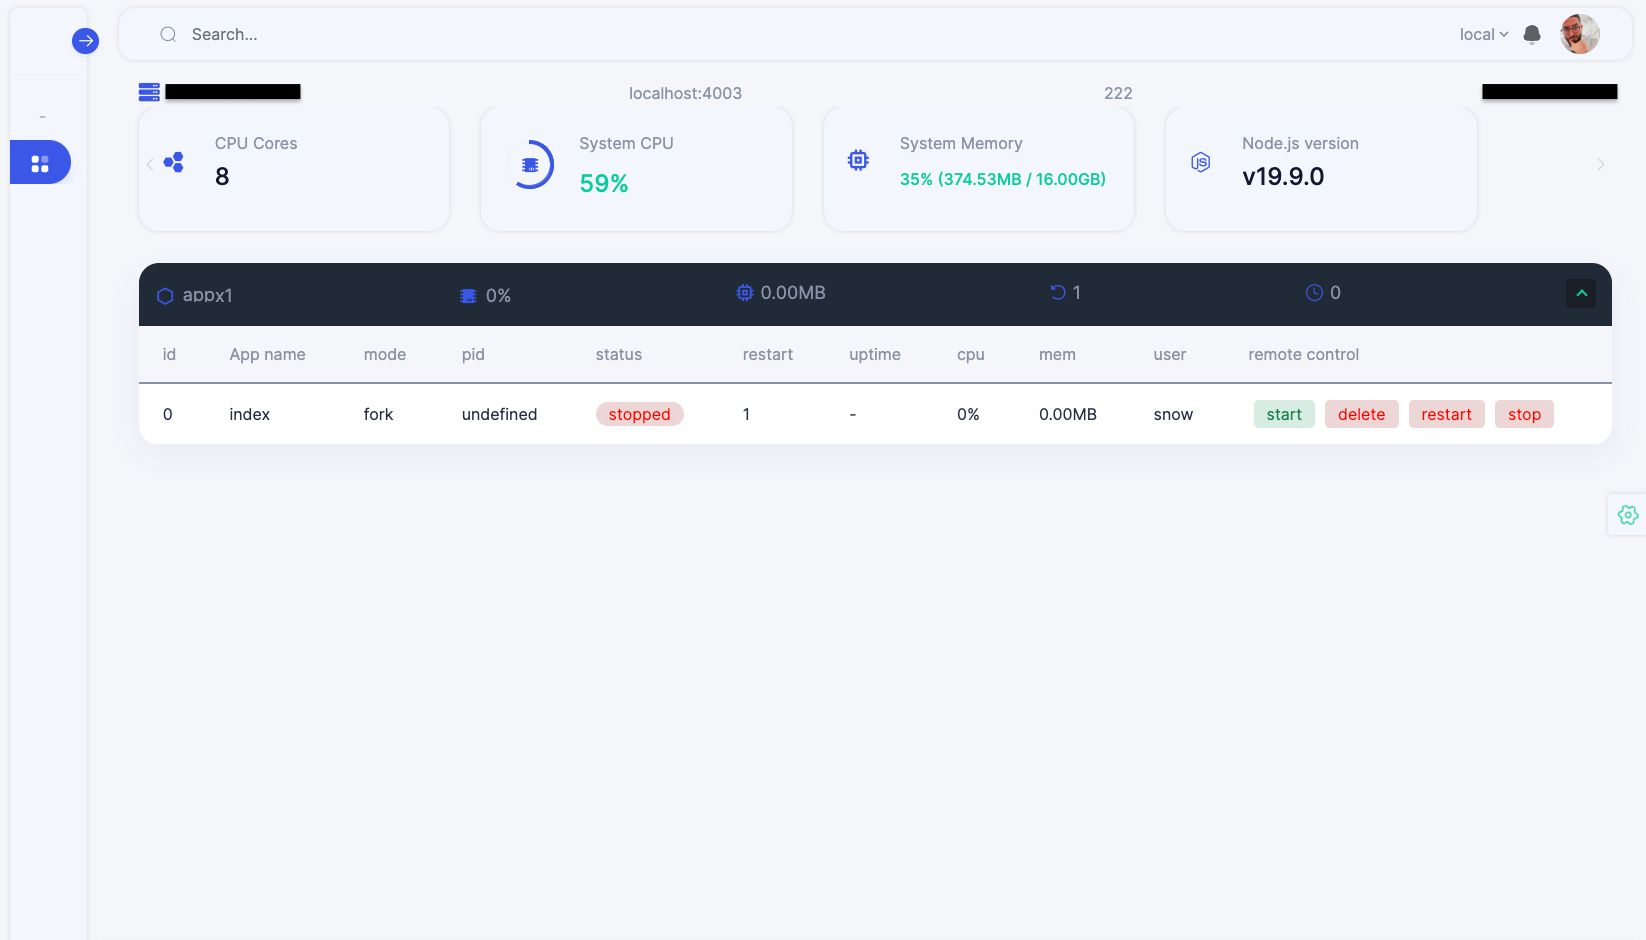
\includegraphics[width=1\textwidth]{img/dashboard.png}
	\caption{Dashboard-Seite (Frontend)}
\end{figure}
\clearpage

	\begin{lstlisting}[caption={VueJs router (Frontend)}, style=js]
		// Dashboard routes
		const dashboardRoutes = (prefix) => [
		  {
			 path: '',
			 name: prefix + '.dashboard',
			 meta: { auth: true, name: 'Home', isBanner: false },
			 component: () => import('@/views/dashboards/IndexPage.vue')
		  }
		]
		// Default routes
		const defaultChildRoutes = (prefix) => [
		  {
			 path: '',
			 name: prefix + '.dashboard',
			 meta: { auth: true, name: 'Home', isBanner: false },
			 component: () => import('@/views/dashboards/IndexPage.vue')
		  },
		  // Spacial Pages
		  {
			 path: '/server',
			 name: prefix + '.server',
			 meta: { auth: true, name: 'Server', isBanner: false },
			 component: () => import('@/views/spacial-pages/serverPage.vue')
		  },
		  {
			 path: '/sensor',
			 name: prefix + '.sensor',
			 meta: { auth: true, name: 'Sensor', isBanner: false },
			 component: () => import('@/views/spacial-pages/sensorPage.vue')
		  },
		  {
			 path: '/setting',
			 name: prefix + '.setting',
			 meta: { auth: true, name: 'Setting', isBanner: false },
			 component: () => import('@/views/spacial-pages/settingPage.vue')
		  },
		  // Users Pages
		  {
			 path: '/sensor-list',
			 name: prefix + '.sensor-list',
			 meta: { auth: true, name: 'Sensor List', isBanner: false },
			 component: () => import('@/views/sensor/ListPage.vue')
		  },
		  {
			 path: '/sensor-add',
			 name: prefix + '.sensor-add',
			 meta: { auth: true, name: 'Sensor Add', isBanner: false },
			 component: () => import('@/views/sensor/AddPage.vue')
		  },
		  {
			 path: '/user-profile',
			 name: prefix + '.user-profile',
			 meta: { auth: true, name: 'User Add', isBanner: false },
			 component: () => import('@/views/user/ProfilePage.vue')
		  },
		  {
			 path: '/charts',
			 name: prefix + '.charts',
			 meta: { auth: true, name: 'Charts', isBanner: false },
			 component: () => import('@/views/charts/charts.vue')
		  },
		  {
			 path: '/validation',
			 name: prefix + '.validation',
			 meta: { auth: true, name: 'Validation', isBanner: false },
			 component: () => import('@/views/forms/ValidationPage.vue')
		  },
		  // Table Pages
		  {
			 path: '/table',
			 name: prefix + '.table',
			 meta: { auth: true, name: 'Table', isBanner: false },
			 component: () => import('@/views/tables/Table.vue')
		  },
		  // Admin Pages
		  {
			 path: '/admin-permissions',
			 name: prefix + '.admin-permissions',
			 meta: { auth: true, name: 'Admin Permissions', isBanner: false },
			 component: () => import('@/views/admin/AdminPage.vue')
		  }
		]

		const errorRoutes = (prefix) => [
		  // Error Pages
		  {
			 path: '404',
			 name: prefix + '.404',
			 meta: { auth: true, name: 'Error 404', isBanner: false },
			 component: () => import('@/views/errors/Error404Page.vue')
		  },
		  {
			 path: '500',
			 name: prefix + '.500',
			 meta: { auth: true, name: 'Error 500', isBanner: false },
			 component: () => import('@/views/errors/Error500Page.vue')
		  },
		  {
			 path: 'maintenance',
			 name: prefix + '.maintenance',
			 meta: { auth: true, name: 'Maintenance', isBanner: false },
			 component: () => import('@/views/errors/MaintenancePage.vue')
		  }
		]
	\end{lstlisting}

\clearpage


	\begin{lstlisting}[caption={registerSensor (Frontend)}, style=js]
		<template>
			<div class="register-sensor">
				<h2>Neuen Sensor registrieren</h2>
				<form @submit.prevent="registerSensor">
					<label for="sensor_name">Sensor Name:</label>
					<input type="text" id="sensor_name" v-model="sensorData.sensor_name" required>
					<label for="sensor_type">Sensor Typ:</label>
					<input type="text" id="sensor_type" v-model="sensorData.sensor_type" required>
					<label for="data_type">Datentyp:</label>
					<input type="text" id="data_type" v-model="sensorData.data_type" required>
					<label for="unit">Einheit:</label>
					<input type="text" id="unit" v-model="sensorData.unit" required>
					<label for="unit_display">Einheitsanzeige:</label>
					<input type="text" id="unit_display" v-model="sensorData.unit_display" required>
					<label for="refresh_interval">Aktualisierungsintervall:</label>
					<input type="text" id="refresh_interval" v-model="sensorData.refresh_interval" required>
					<label for="data_source">Datenquelle:</label>
					<input type="text" id="data_source" v-model="sensorData.data_source" required>
					<label for="data_parser">Daten-Parser:</label>
					<input type="text" id="data_parser" v-model="sensorData.data_parser" required>
					<label for="sensor_max">Maximalwert:</label>
					<input type="text" id="sensor_max" v-model="sensorData.sensor_max" required>
					<label for="sensor_min">Minimalwert:</label>
					<input type="text" id="sensor_min" v-model="sensorData.sensor_min" required>
					<label for="visible">Sichtbarkeit:</label>
					<input type="checkbox" id="visible" v-model="sensorData.visible">
					<label for="data">Daten:</label>
					<textarea id="data" v-model="sensorData.Data"></textarea>
					<label for="show">Anzeigen:</label>
					<input type="checkbox" id="show" v-model="sensorData.show">
					<label for="saveData">Daten speichern:</label>
					<input type="checkbox" id="saveData" v-model="sensorData.saveData">
					<label for="DataRetentionPeriodInMonths">Datenspeicherzeit:</label>
					<input type="text" id="DataRetentionPeriodInMonths" v-model="sensorData.DataRetentionPeriodInMonths" required>
					<button type="submit">Sensor registrieren</button>
				</form>
				<div v-if="errorMessage" class="error-message">{{ errorMessage }}</div>
				<div v-if="successMessage" class="success-message">{{ successMessage }}</div>
			</div>
		</template>

		<script>
		export default {
		  data() {
			 return {
				// Hier kommen die Formularfelder als data-Properties hin
				sensor_name: "",
				sensor_type: "",
				data_type: "",
				unit: "",
				unit_display: "",
				refresh_interval: "",
				data_source: "",
				data_parser: "",
				sensor_max: "",
				sensor_min: "",
				visible: "",
				Data: "",
				show: "",
				saveData: "",
				DataRetentionPeriodInMonths: "",
			 };
		  },
		  methods: {
			 async registerSensor() {
				// Erstelle das Sensorobjekt mit den Formulardaten
				const sensorData = {
				  sensor_name: this.sensor_name,
				  sensor_type: this.sensor_type,
				  data_type: this.data_type,
				  unit: this.unit,
				  unit_display: this.unit_display,
				  refresh_interval: this.refresh_interval,
				  data_source: this.data_source,
				  data_parser: this.data_parser,
				  sensor_max: this.sensor_max,
				  sensor_min: this.sensor_min,
				  visible: this.visible,
				  Data: this.Data,
				  show: this.show,
				  saveData: this.saveData,
				  DataRetentionPeriodInMonths: this.DataRetentionPeriodInMonths,
				};

				try {
				  // Sende das Sensorobjekt an den Server
				  const response = await axios.post("/registerSensor", sensorData);

				  // Wenn die Sensorregistrierung erfolgreich war, zeige eine Erfolgsmeldung an
				  if (response.data.code === 207) {
					 alert(`Sensor erfolgreich registriert mit ID ${response.data.sensor_id}`);
				  }
				} catch (error) {
				  // Wenn es einen Fehler gab, zeige eine Fehlermeldung an
				  alert("Fehler beim Registrieren des Sensors");
				  console.error(error);
				}
			 },
		  },
		};
		</script>
	\end{lstlisting}

	\begin{lstlisting}[caption={sort Function (Frontend)}, style=js]
	/* Used to sort the data.
		This function sorts an array of objects by a given property, either in ascending or descending order.
		It also converts any dates in the given property to ISO format before sorting,
		and converts them back to the original format after sorting.
		*/
const sortByProperty = (arr, prop, sortOrder, nullText) =>
{
	log(arr, prop, sortOrder, nullText);
	try {
		if (arr == null || arr.length <= 0) return false;
		if (prop == null || prop.length <= 0) return false;
		if (sortOrder == null || sortOrder.length <= 0) return false;
		const dateRegex = /(\d{1,2})\.(\d{1,2})\.(\d{4}) (\d{1,2}):(\d{1,2}):(\d{1,2})/;
		let isDate = false;
		sortOrder = sortOrder === 'asc' ? true : false;
		let resultsArray = [];
		let y = 0;
		// convert date format in object array to ISO format
		if (arr[y][prop] === nullText) y++;
		if (typeof arr[y][prop] === 'string') {
			// if (isNaN(arr[0][prop])) {
			if (arr[y] && arr[y][prop] && arr[y][prop].match(dateRegex)) {
				arr.forEach((e) => {
					var match = e[prop].match(dateRegex);
					if (match) {
						e[prop] = isoDate(match);
						isDate = true;
					}
				});
			}
			// }
		} else {
			if (isNaN(arr[y][prop].value)) {
				if (arr[y] && arr[y][prop].value && arr[y][prop].value.match(dateRegex)) {
					arr.forEach((e) => {
						var match = e[prop].value.match(dateRegex);
						if (match) {
							e[prop].value = isoDate(match);
							isDate = true;
						}
					});
				}
			}
		}
		// Sortieren des Arrays nach der Eigenschaft und der Sortierreihenfolge.
		//sorts the array of objects by the specified property
		//first checks if the value of the property is a string, if so it transforms it to lowercase
		//if the value is an object, it gets the value property
		//if the value is a number, it sorts it as a number
		//if the value is a string, it checks if it has a currency symbol, if so it parses it to a float and sorts it as a number
		//if the value is a string, it sorts it as a string

		resultsArray = arr.sort((a, b) => {
			var aValue = typeof a[ prop ] === 'string' ? a[ prop ].toLowerCase() : a[ prop ];
			var bValue = typeof b[ prop ] === 'string' ? b[ prop ].toLowerCase() : b[ prop ];
			aValue = typeof aValue === 'object' ? aValue.value : aValue;
			bValue = typeof bValue === 'object' ? bValue.value : bValue;

			if (!isNaN(aValue) && !isNaN(bValue)) {
				return sortOrder ? aValue - bValue : bValue - aValue;
			} else if (typeof aValue === 'string' && typeof bValue === 'string') {
				return sortOrder ? aValue.localeCompare(bValue) : bValue.localeCompare(aValue);
			} else {
				return sortOrder ? aValue.localeCompare(bValue) : bValue.localeCompare(aValue);
			}
		});

		if (isDate) {
			resultsArray.forEach((e) => {
				typeof e[prop] === 'string' ? (e[prop] = convertIsoToGermanDate(e[prop])) : (e[prop].value = convertIsoToGermanDate(e[prop].value));
			});
		}
		return resultsArray;
	} catch (error) {
		console.error(error);
	}
};

// This function converts an isoDate to a german date format
const convertIsoToGermanDate = (isoDate) => {
	try {
		// Create a new Date object from the isoDate
		const date = new Date(isoDate);
		// Extract the date, month, and year from the date object
		const day = date.getDate().toString().padStart(2, '0');
		const month = (date.getMonth() + 1).toString().padStart(2, '0');
		const year = date.getFullYear().toString();
		// Extract the hours, minutes, and seconds from the date object
		const hours = date.getHours().toString().padStart(2, '0');
		const minutes = date.getMinutes().toString().padStart(2, '0');
		const seconds = date.getSeconds().toString().padStart(2, '0');
		// Return the date with the format dd.mm.yyyy hh:mm:ss
		return `${day}.${month}.${year} ${hours}:${minutes}:${seconds}`;
	} catch (error) {
		console.error(error);
	}
};

// This function converts a date from the format DD/MM/YYYY to the format YYYY-MM-DD.
const isoDate = (match) => {
	try {
		const year = match[3];
		const month = match[2];
		const day = match[1];
		const hours = match[4];
		const minutes = match[5];
		const seconds = match[6];
		return `${year}-${month}-${day}T${hours}:${minutes}:${seconds}`;
	} catch (error) {
		console.error(error);
	}
};

const sortArrayBasedOnReference = (arrayA, arrayB) => {
	return arrayB.sort((a, b) => {
		const aIndex = arrayA.indexOf(a.text);
		const bIndex = arrayA.indexOf(b.text);

		if (aIndex === -1) {
			return 1;
		}

		if (bIndex === -1) {
			return -1;
		}

		return aIndex - bIndex;
	});
};

const sortArrayByReferenceArray = (arrayA, referenceArray) => {
	const sortedArrayA = new Array(arrayA.length);

	for (const element of referenceArray) {
		const indexInArrayA = arrayA.indexOf(element.text);

		if (indexInArrayA !== -1) {
			sortedArrayA[element.index] = element.text;
		}
	}

	return sortedArrayA.filter((element) => element !== undefined);
};

const mergeArrayBIntoArrayA = (arrayA, arrayB) => {
	const newArrayA = [];

	for (const element of arrayB) {
		const indexInArrayA = arrayA.indexOf(element.text);
		if (indexInArrayA !== -1) {
			newArrayA.push(element.text);
		}
	}

	for (const element of arrayA) {
		if (!newArrayA.includes(element)) {
			newArrayA.push(element);
		}
	}

	return newArrayA;
};
\end{lstlisting}
\begin{lstlisting}[caption={search Function (Frontend)}, style=js]
const search = (lst, searchLst) => {
	try {
		for (let i = 0; i < searchLst.length; i++) {
			const element = searchLst[i];
			/* Searching in a nested object. */
			lst = filterNode(lst, element.Property, element.Text);
		}
		return lst;
	} catch (error) {
		console.error(error);
	}
};

var canSplit = (str, elements) => {
	try {
		var lst = {
			methor: [],
			str: [],
		};
		for (var i = 0; i < elements.length; i++) {
			if ((str || '').split(elements[i]).length > 1) {
				lst.methor.push(elements[i]);
				lst.str.push(str.split(elements[i]));
			}
		}
		return lst;
	} catch (error) {
		console.error(error);
	}
};

const filterNode = (nodes, parts, searchText) => {
	try {
		if (searchText === 'null') searchText = ' ';
		var lst = [];
		log(parts);
		parts = parts.split('.'); //! you must not have . in the propati
		searchText = searchText.split('&');
		if (typeof nodes == 'undefined' && typeof nodes != 'object') {
			console.error('nodes is not an object');
			return;
		}
		for (let k = 0; k < nodes.length; k++) {
			const e = nodes[k];
			/* Getting the keys of the object. */
			let keys = Object.keys(e);
			var x = 0;
			for (let i = 0; i < keys.length; i++) {
				var key = keys[i];
				if (typeof key == 'object') {
					if (typeof keys[i] == 'object') {
						let sublst = filterNode(e[keys[i]], parts[x], searchText);
						 if (sublst != null) {
						 	sublst.forEach((x) => {
						 		lst.push(x);
						 	});
						 }
					}
				} else {
					if (key == parts[x]) {
						var lNode = typeof e[key] == 'object' ? e[key].value : e[key];
						if (lNode == null) {
							if (searchInSubNode(lNode, searchText, parts, x)) {
								lst.push(e);
							}
						} else {
							if (typeof searchText == 'string') {
								if (searchInNode(lNode, searchText)) {
									lst.push(e);
								}
							} else {
								searchText.forEach((element) => {
									if (searchInNode(lNode, element)) {
										lst.push(e);
									}
								});
							}
						}
					}
				}
			}
		}
		return lst;
	} catch (error) {
		console.error(error);
	}
};

// Search in a subnode
/* Searching in a nested object. */
searchInSubNode = (items, searchText, parts, x) => {
	try {
		if (items != null) {
			++x;
			for (let y = 0; y < items.length; y++) {
				const element = items[y];
				var lNodeText = element[parts[x]];
				if (lNodeText != null && typeof lNodeText == 'string') {
					lNodeText = lNodeText.toLowerCase();
					if (lNodeText.includes(searchText)) {
						return true;
					}
				} else if (typeof lNodeText == 'object') {
					if (searchInSubNode(lNodeText, searchText, parts, x)) {
						return true;
					}
				}
			}
		}
		return false;
	} catch (error) {
		console.error(error);
	}
};

/* This function is used to search in a nested object. */
searchInNode = (item, searchText) => {
	try {
		item = String(item);
		/* Converting the item to lower case. */
		item = item.toLowerCase();
		/* Checking if the searchText is in the item. */
		if (typeof searchText == 'string') {
			if (item.includes(searchText.toLowerCase())) {
				return true;
			}
		}
		return false;
	} catch (error) {
		console.error(error);
	}
};
\end{lstlisting}


\clearpage
